\documentclass[11pt]{article}
\usepackage[textwidth=18.0cm, textheight=23.0cm, top=2.0cm]{geometry}
\usepackage{pst-all}
\usepackage{amssymb}
\usepackage{tikz}
\usepackage{underscore}\begin{document}
\pagestyle{empty}


ClassName: \underline{\textbf{Class_08.2bp-32}}
\par
BinSize: \underline{\textbf{100 × 100}}
\par
ReduceSize: \underline{\textbf{100 × 100}}
\par
TypeNum: \underline{\textbf{80}}
\par
Num: \underline{\textbf{80}}
\par
OutS: \underline{\textbf{210000}}
\par
InS: \underline{\textbf{173150}}
\par
Rate: \underline{\textbf{0.825}}
\par
UB: \underline{\textbf{21}}
\par
LB0: \underline{\textbf{20}}
\par
LB: \underline{\textbf{21}}
\par
LBWithCut: \underline{\textbf{21}}
\par
NodeCut: \underline{\textbf{0}}
\par
ExtendedNodeCnt: \underline{\textbf{1}}
\par
GenNodeCnt: \underline{\textbf{1}}
\par
PrimalNode: \underline{\textbf{0}}
\par
ColumnCount: \underline{\textbf{177}}
\par
TotalCutCount: \underline{\textbf{0}}
\par
RootCutCount: \underline{\textbf{0}}
\par
LPSolverCnt: \underline{\textbf{157}}
\par
PricingSolverCnt: \underline{\textbf{157}}
\par
BranchAndBoundNum: \underline{\textbf{1}}
\par
isOpt: \underline{\textbf{true}}
\par
TimeOnPrimal: \underline{\textbf{0.000 s}}
\par
TimeOnPricing: \underline{\textbf{18.636 s}}
\par
TimeOnRmp: \underline{\textbf{0.168 s}}
\par
TotalTime: \underline{\textbf{18.927 s}}
\par
\newpage


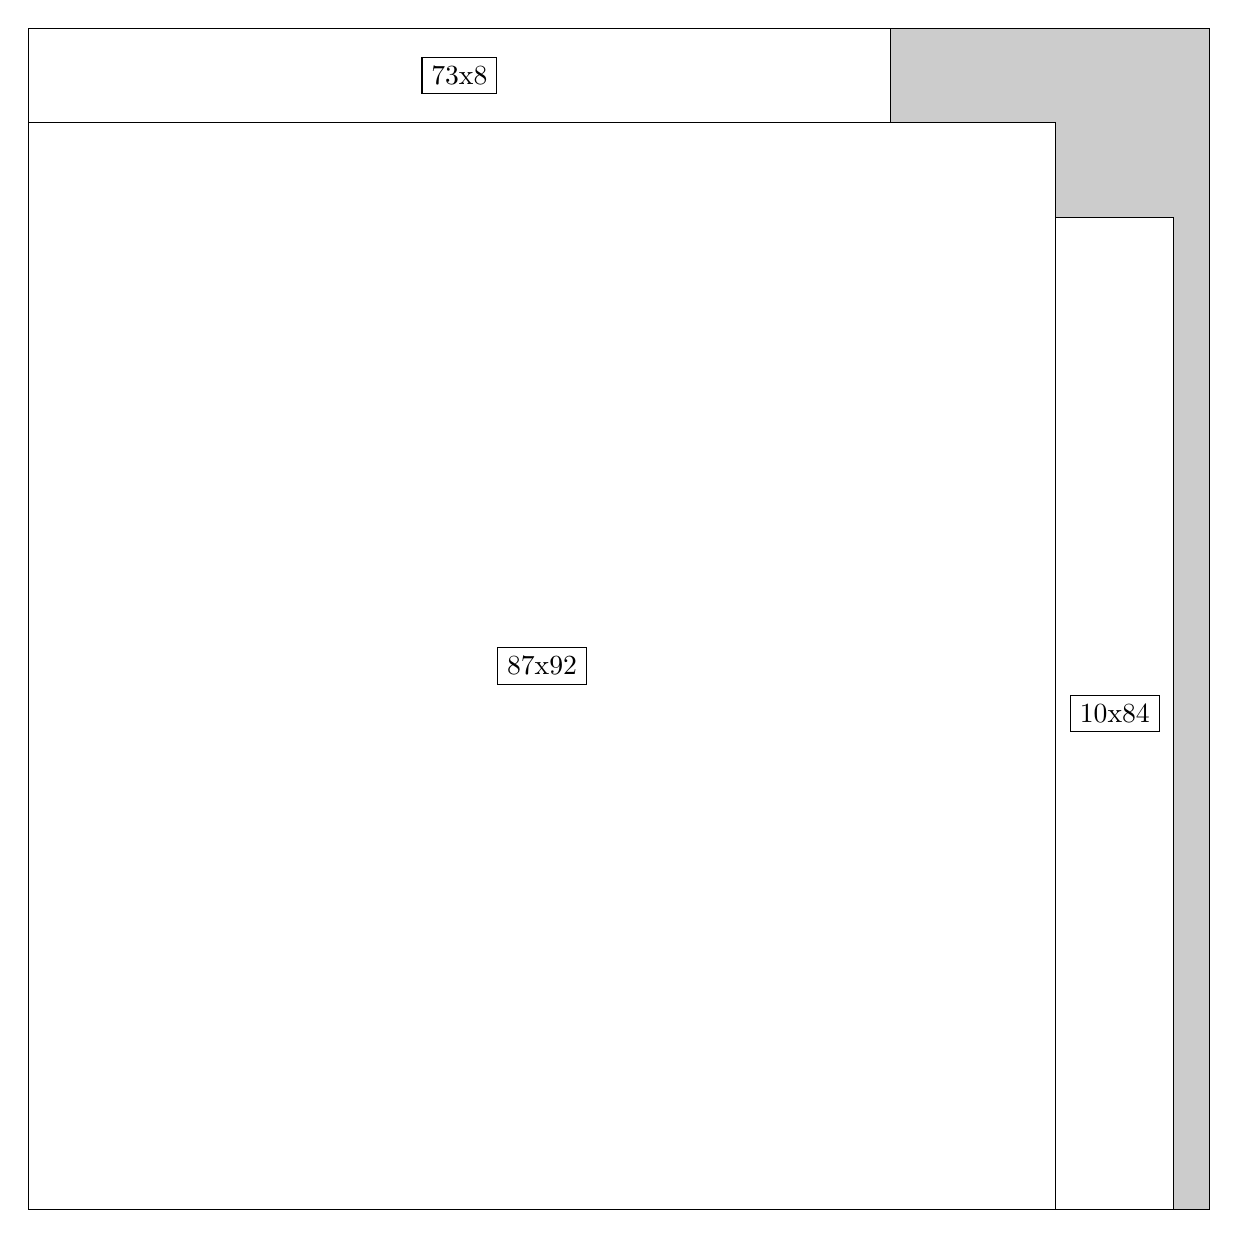
\begin{tikzpicture}[shorten >=1pt,scale=1.0,every node/.style={scale=1.0},->]
\tikzstyle{vertex}=[circle,fill=black!25,minimum size=14pt,inner sep=0pt]
\filldraw[fill=gray!40!white, draw=black] (0,0) rectangle (15.0,15.0);
\foreach \name/\x/\y/\w/\h in {87x92/0.0/0.0/13.049999999999999/13.799999999999999,10x84/13.049999999999999/0.0/1.5/12.6,73x8/0.0/13.799999999999999/10.95/1.2}
\filldraw[fill=white!40!white, draw=black] (\x,\y) rectangle node[draw] (\name) {\name} ++(\w,\h);
\end{tikzpicture}


w =87 , h =92 , x =0 , y =0 , v =8004
\par
w =10 , h =84 , x =87 , y =0 , v =840
\par
w =73 , h =8 , x =0 , y =92 , v =584
\par
\newpage


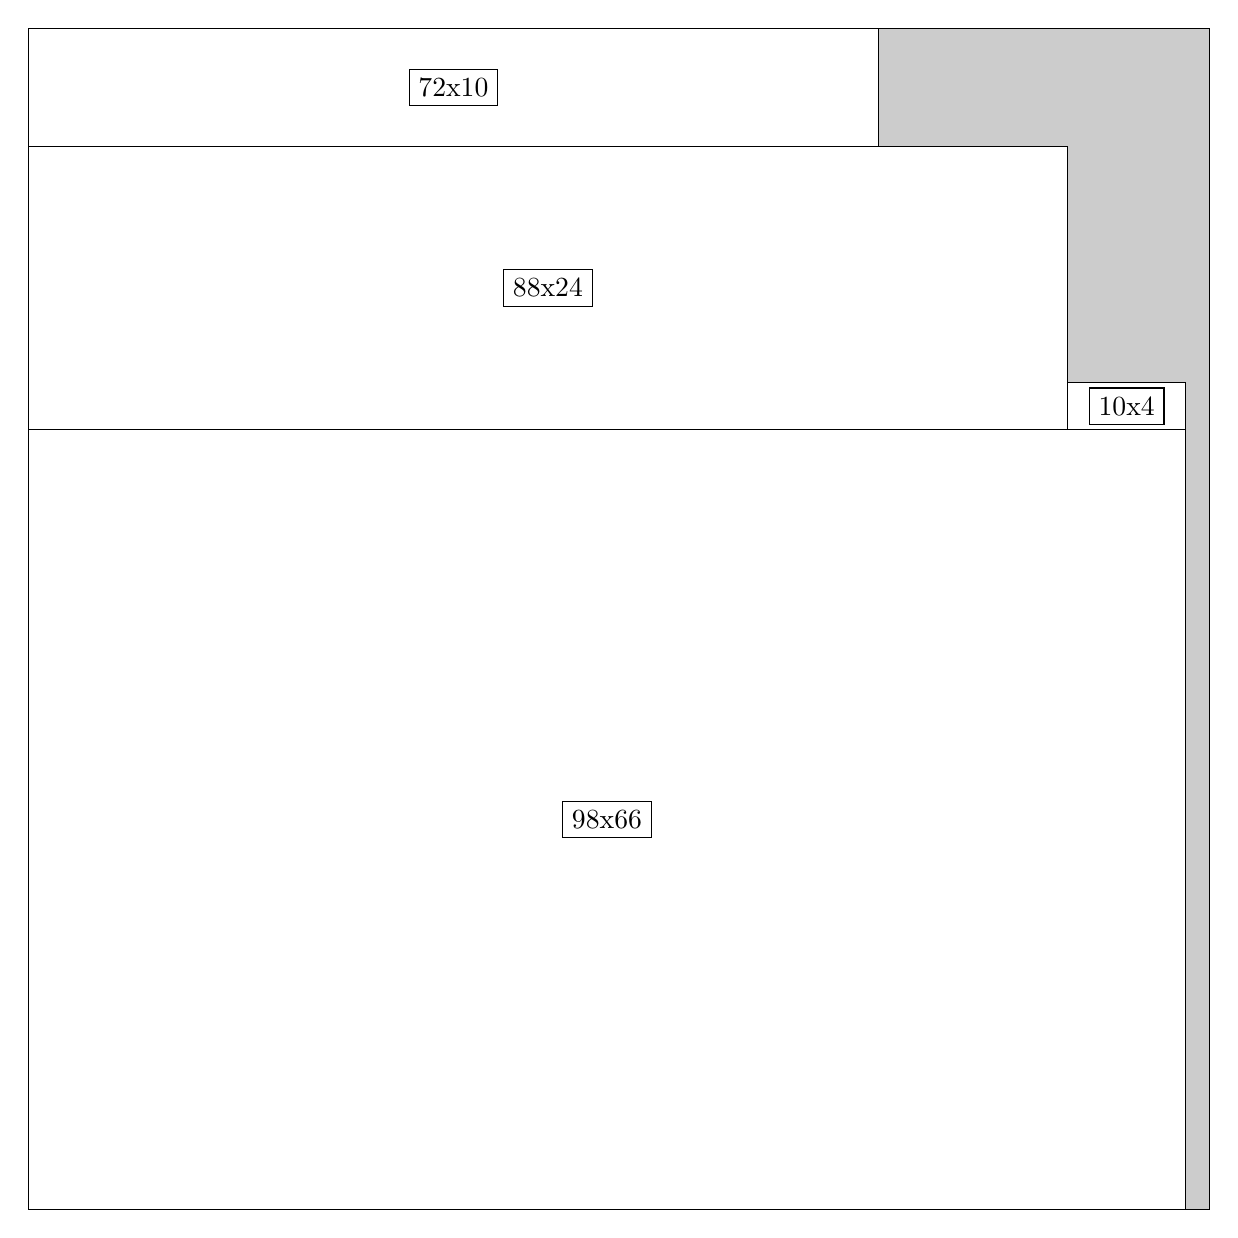
\begin{tikzpicture}[shorten >=1pt,scale=1.0,every node/.style={scale=1.0},->]
\tikzstyle{vertex}=[circle,fill=black!25,minimum size=14pt,inner sep=0pt]
\filldraw[fill=gray!40!white, draw=black] (0,0) rectangle (15.0,15.0);
\foreach \name/\x/\y/\w/\h in {98x66/0.0/0.0/14.7/9.9,88x24/0.0/9.9/13.2/3.5999999999999996,72x10/0.0/13.5/10.799999999999999/1.5,10x4/13.2/9.9/1.5/0.6}
\filldraw[fill=white!40!white, draw=black] (\x,\y) rectangle node[draw] (\name) {\name} ++(\w,\h);
\end{tikzpicture}


w =98 , h =66 , x =0 , y =0 , v =6468
\par
w =88 , h =24 , x =0 , y =66 , v =2112
\par
w =72 , h =10 , x =0 , y =90 , v =720
\par
w =10 , h =4 , x =88 , y =66 , v =40
\par
\newpage


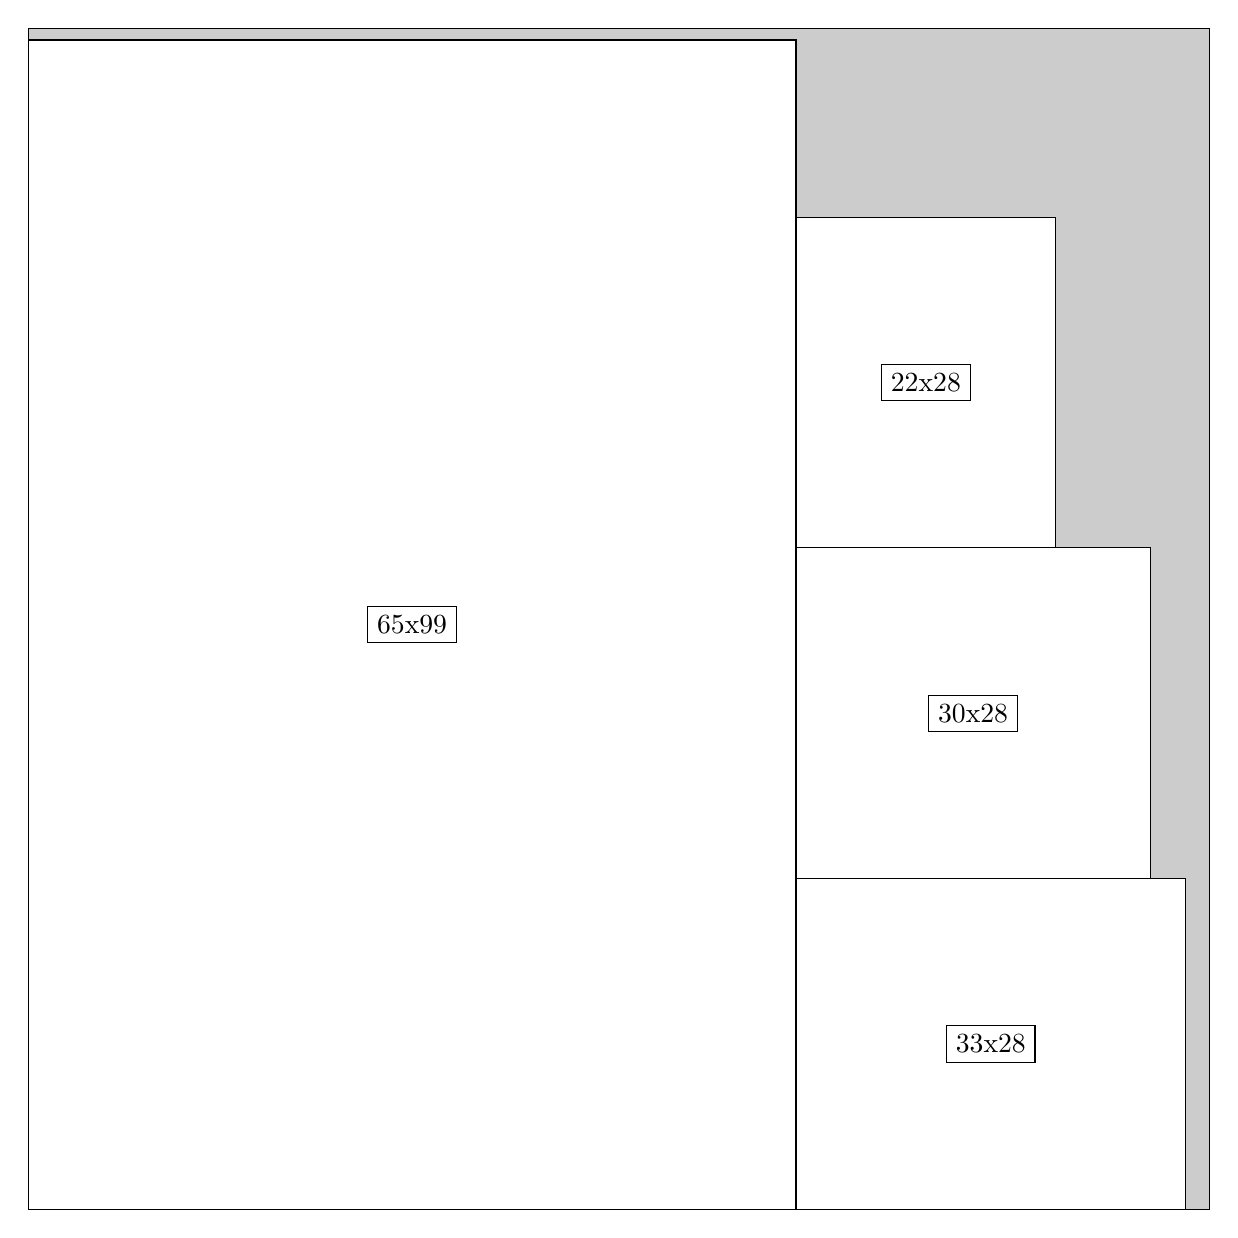
\begin{tikzpicture}[shorten >=1pt,scale=1.0,every node/.style={scale=1.0},->]
\tikzstyle{vertex}=[circle,fill=black!25,minimum size=14pt,inner sep=0pt]
\filldraw[fill=gray!40!white, draw=black] (0,0) rectangle (15.0,15.0);
\foreach \name/\x/\y/\w/\h in {65x99/0.0/0.0/9.75/14.85,33x28/9.75/0.0/4.95/4.2,30x28/9.75/4.2/4.5/4.2,22x28/9.75/8.4/3.3/4.2}
\filldraw[fill=white!40!white, draw=black] (\x,\y) rectangle node[draw] (\name) {\name} ++(\w,\h);
\end{tikzpicture}


w =65 , h =99 , x =0 , y =0 , v =6435
\par
w =33 , h =28 , x =65 , y =0 , v =924
\par
w =30 , h =28 , x =65 , y =28 , v =840
\par
w =22 , h =28 , x =65 , y =56 , v =616
\par
\newpage


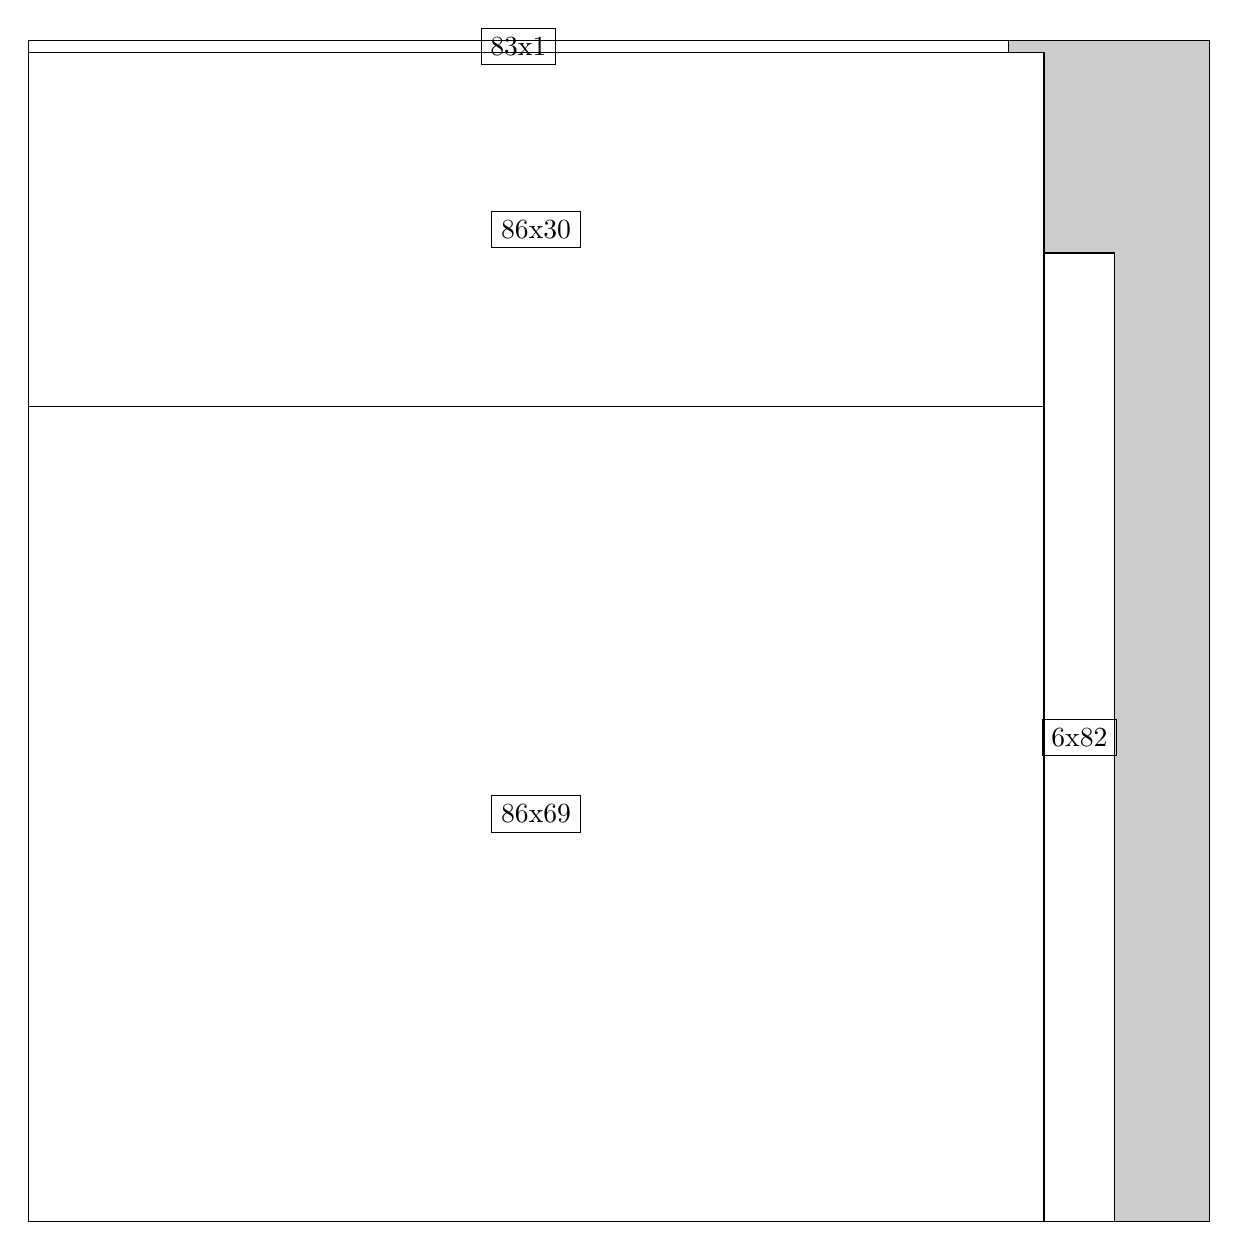
\begin{tikzpicture}[shorten >=1pt,scale=1.0,every node/.style={scale=1.0},->]
\tikzstyle{vertex}=[circle,fill=black!25,minimum size=14pt,inner sep=0pt]
\filldraw[fill=gray!40!white, draw=black] (0,0) rectangle (15.0,15.0);
\foreach \name/\x/\y/\w/\h in {86x69/0.0/0.0/12.9/10.35,86x30/0.0/10.35/12.9/4.5,6x82/12.9/0.0/0.8999999999999999/12.299999999999999,83x1/0.0/14.85/12.45/0.15}
\filldraw[fill=white!40!white, draw=black] (\x,\y) rectangle node[draw] (\name) {\name} ++(\w,\h);
\end{tikzpicture}


w =86 , h =69 , x =0 , y =0 , v =5934
\par
w =86 , h =30 , x =0 , y =69 , v =2580
\par
w =6 , h =82 , x =86 , y =0 , v =492
\par
w =83 , h =1 , x =0 , y =99 , v =83
\par
\newpage


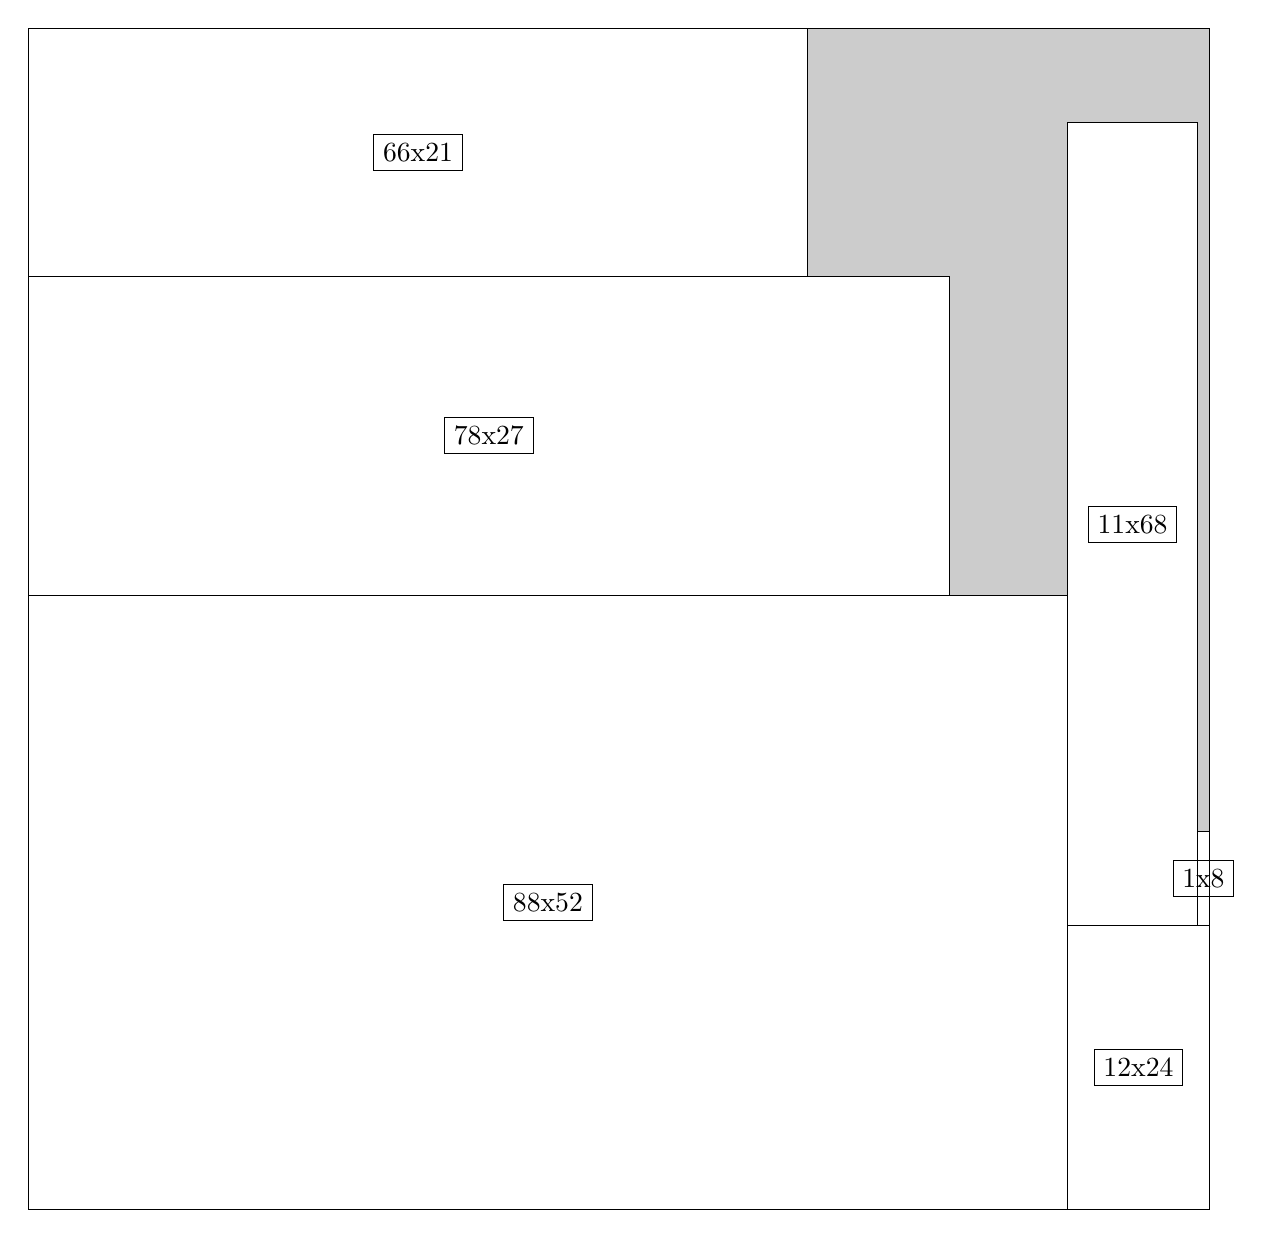
\begin{tikzpicture}[shorten >=1pt,scale=1.0,every node/.style={scale=1.0},->]
\tikzstyle{vertex}=[circle,fill=black!25,minimum size=14pt,inner sep=0pt]
\filldraw[fill=gray!40!white, draw=black] (0,0) rectangle (15.0,15.0);
\foreach \name/\x/\y/\w/\h in {88x52/0.0/0.0/13.2/7.8,11x68/13.2/3.5999999999999996/1.65/10.2,78x27/0.0/7.8/11.7/4.05,66x21/0.0/11.85/9.9/3.15,12x24/13.2/0.0/1.7999999999999998/3.5999999999999996,1x8/14.85/3.5999999999999996/0.15/1.2}
\filldraw[fill=white!40!white, draw=black] (\x,\y) rectangle node[draw] (\name) {\name} ++(\w,\h);
\end{tikzpicture}


w =88 , h =52 , x =0 , y =0 , v =4576
\par
w =11 , h =68 , x =88 , y =24 , v =748
\par
w =78 , h =27 , x =0 , y =52 , v =2106
\par
w =66 , h =21 , x =0 , y =79 , v =1386
\par
w =12 , h =24 , x =88 , y =0 , v =288
\par
w =1 , h =8 , x =99 , y =24 , v =8
\par
\newpage


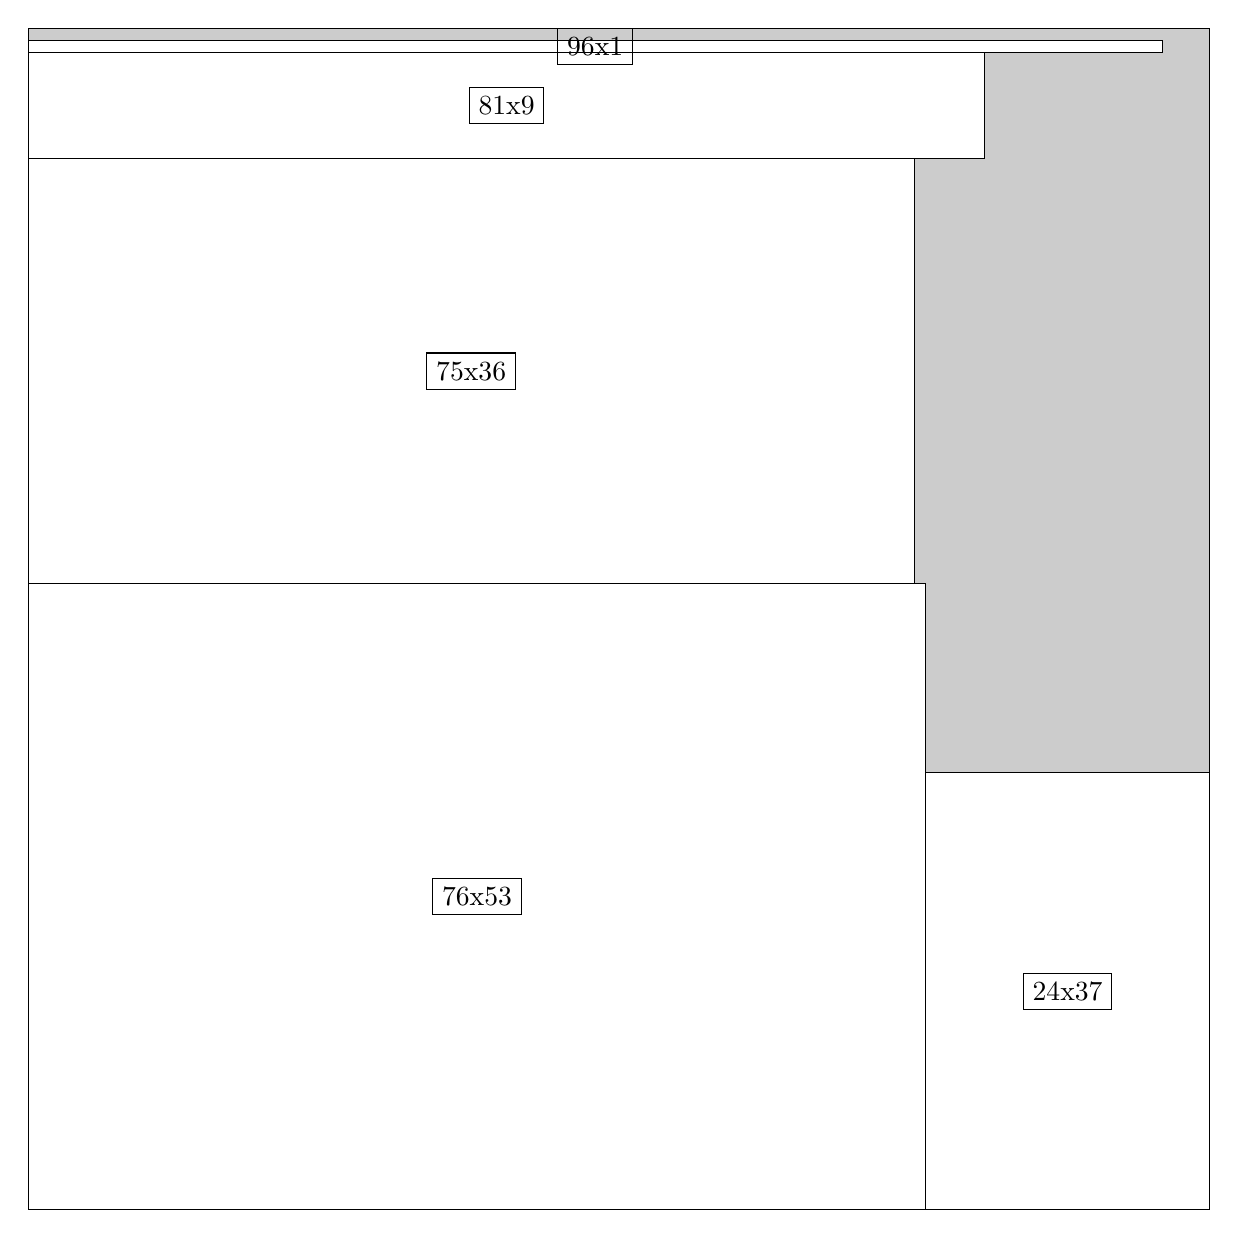
\begin{tikzpicture}[shorten >=1pt,scale=1.0,every node/.style={scale=1.0},->]
\tikzstyle{vertex}=[circle,fill=black!25,minimum size=14pt,inner sep=0pt]
\filldraw[fill=gray!40!white, draw=black] (0,0) rectangle (15.0,15.0);
\foreach \name/\x/\y/\w/\h in {76x53/0.0/0.0/11.4/7.949999999999999,75x36/0.0/7.949999999999999/11.25/5.3999999999999995,24x37/11.4/0.0/3.5999999999999996/5.55,81x9/0.0/13.35/12.15/1.3499999999999999,96x1/0.0/14.7/14.399999999999999/0.15}
\filldraw[fill=white!40!white, draw=black] (\x,\y) rectangle node[draw] (\name) {\name} ++(\w,\h);
\end{tikzpicture}


w =76 , h =53 , x =0 , y =0 , v =4028
\par
w =75 , h =36 , x =0 , y =53 , v =2700
\par
w =24 , h =37 , x =76 , y =0 , v =888
\par
w =81 , h =9 , x =0 , y =89 , v =729
\par
w =96 , h =1 , x =0 , y =98 , v =96
\par
\newpage


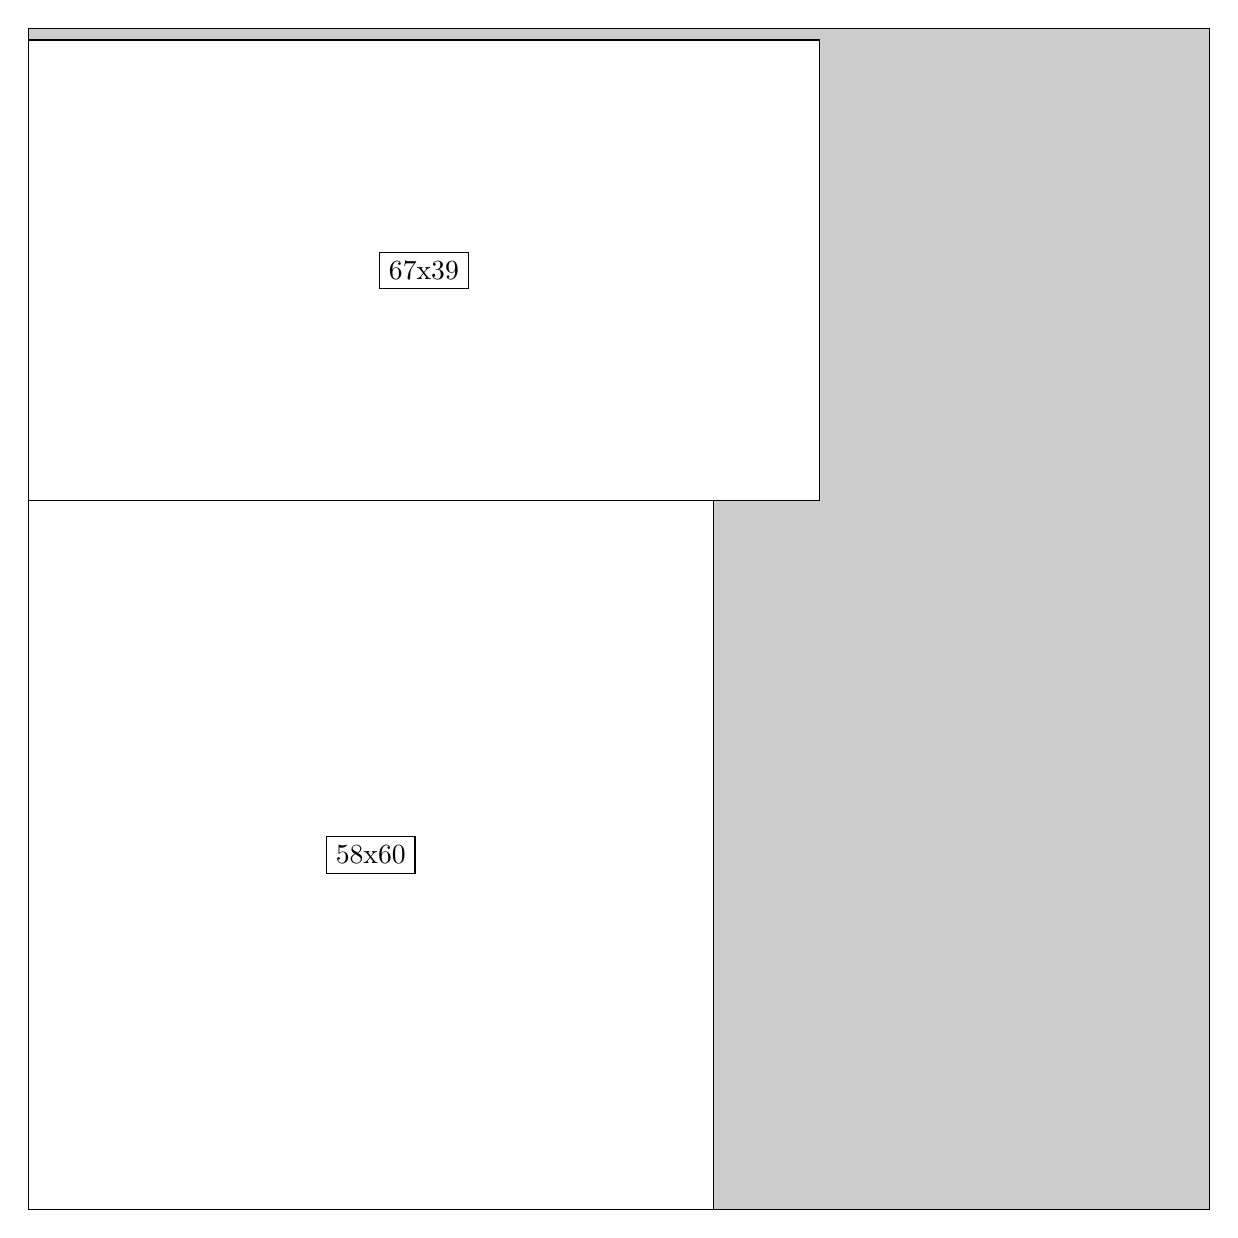
\begin{tikzpicture}[shorten >=1pt,scale=1.0,every node/.style={scale=1.0},->]
\tikzstyle{vertex}=[circle,fill=black!25,minimum size=14pt,inner sep=0pt]
\filldraw[fill=gray!40!white, draw=black] (0,0) rectangle (15.0,15.0);
\foreach \name/\x/\y/\w/\h in {58x60/0.0/0.0/8.7/9.0,67x39/0.0/9.0/10.049999999999999/5.85}
\filldraw[fill=white!40!white, draw=black] (\x,\y) rectangle node[draw] (\name) {\name} ++(\w,\h);
\end{tikzpicture}


w =58 , h =60 , x =0 , y =0 , v =3480
\par
w =67 , h =39 , x =0 , y =60 , v =2613
\par
\newpage


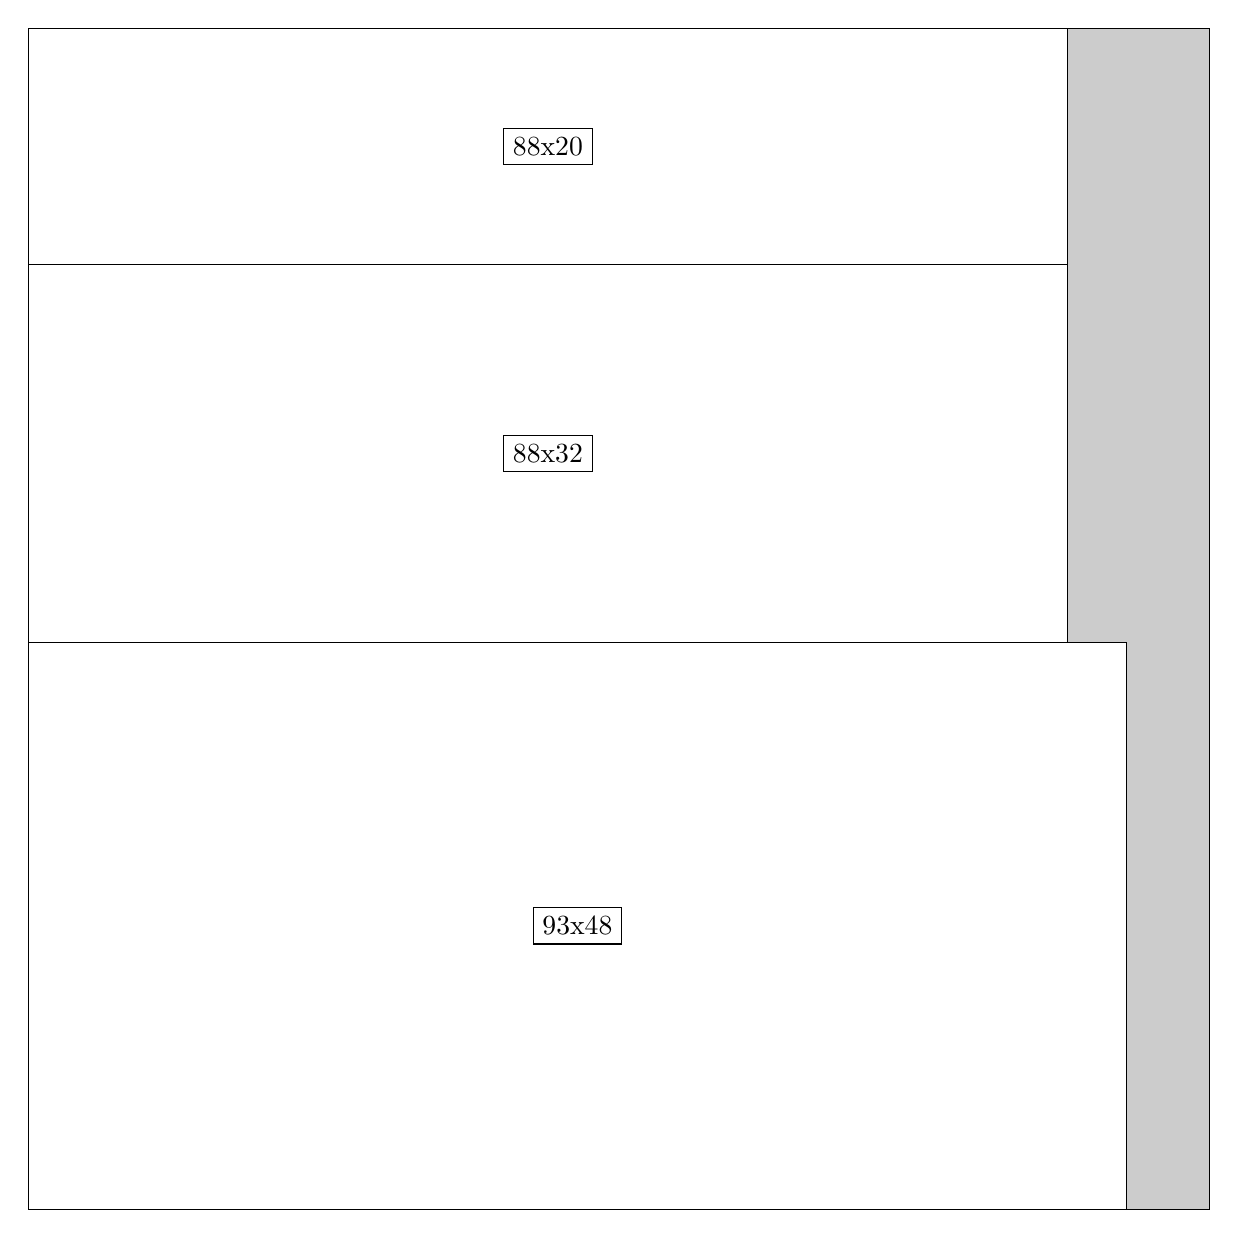
\begin{tikzpicture}[shorten >=1pt,scale=1.0,every node/.style={scale=1.0},->]
\tikzstyle{vertex}=[circle,fill=black!25,minimum size=14pt,inner sep=0pt]
\filldraw[fill=gray!40!white, draw=black] (0,0) rectangle (15.0,15.0);
\foreach \name/\x/\y/\w/\h in {93x48/0.0/0.0/13.95/7.199999999999999,88x32/0.0/7.199999999999999/13.2/4.8,88x20/0.0/12.0/13.2/3.0}
\filldraw[fill=white!40!white, draw=black] (\x,\y) rectangle node[draw] (\name) {\name} ++(\w,\h);
\end{tikzpicture}


w =93 , h =48 , x =0 , y =0 , v =4464
\par
w =88 , h =32 , x =0 , y =48 , v =2816
\par
w =88 , h =20 , x =0 , y =80 , v =1760
\par
\newpage


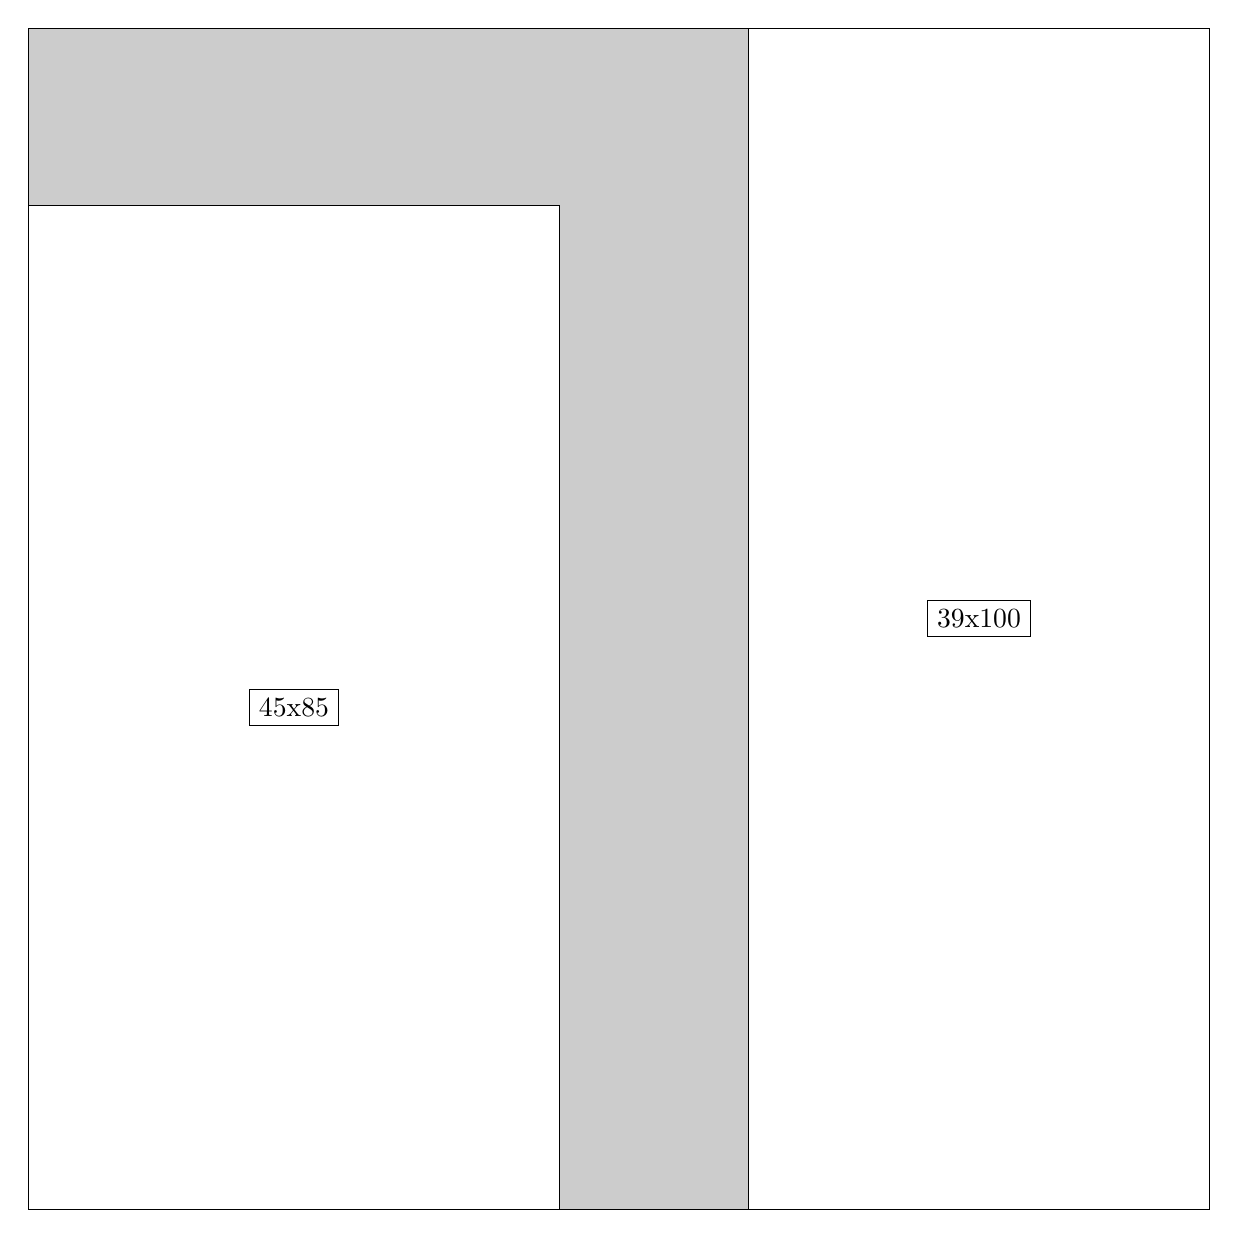
\begin{tikzpicture}[shorten >=1pt,scale=1.0,every node/.style={scale=1.0},->]
\tikzstyle{vertex}=[circle,fill=black!25,minimum size=14pt,inner sep=0pt]
\filldraw[fill=gray!40!white, draw=black] (0,0) rectangle (15.0,15.0);
\foreach \name/\x/\y/\w/\h in {39x100/9.15/0.0/5.85/15.0,45x85/0.0/0.0/6.75/12.75}
\filldraw[fill=white!40!white, draw=black] (\x,\y) rectangle node[draw] (\name) {\name} ++(\w,\h);
\end{tikzpicture}


w =39 , h =100 , x =61 , y =0 , v =3900
\par
w =45 , h =85 , x =0 , y =0 , v =3825
\par
\newpage


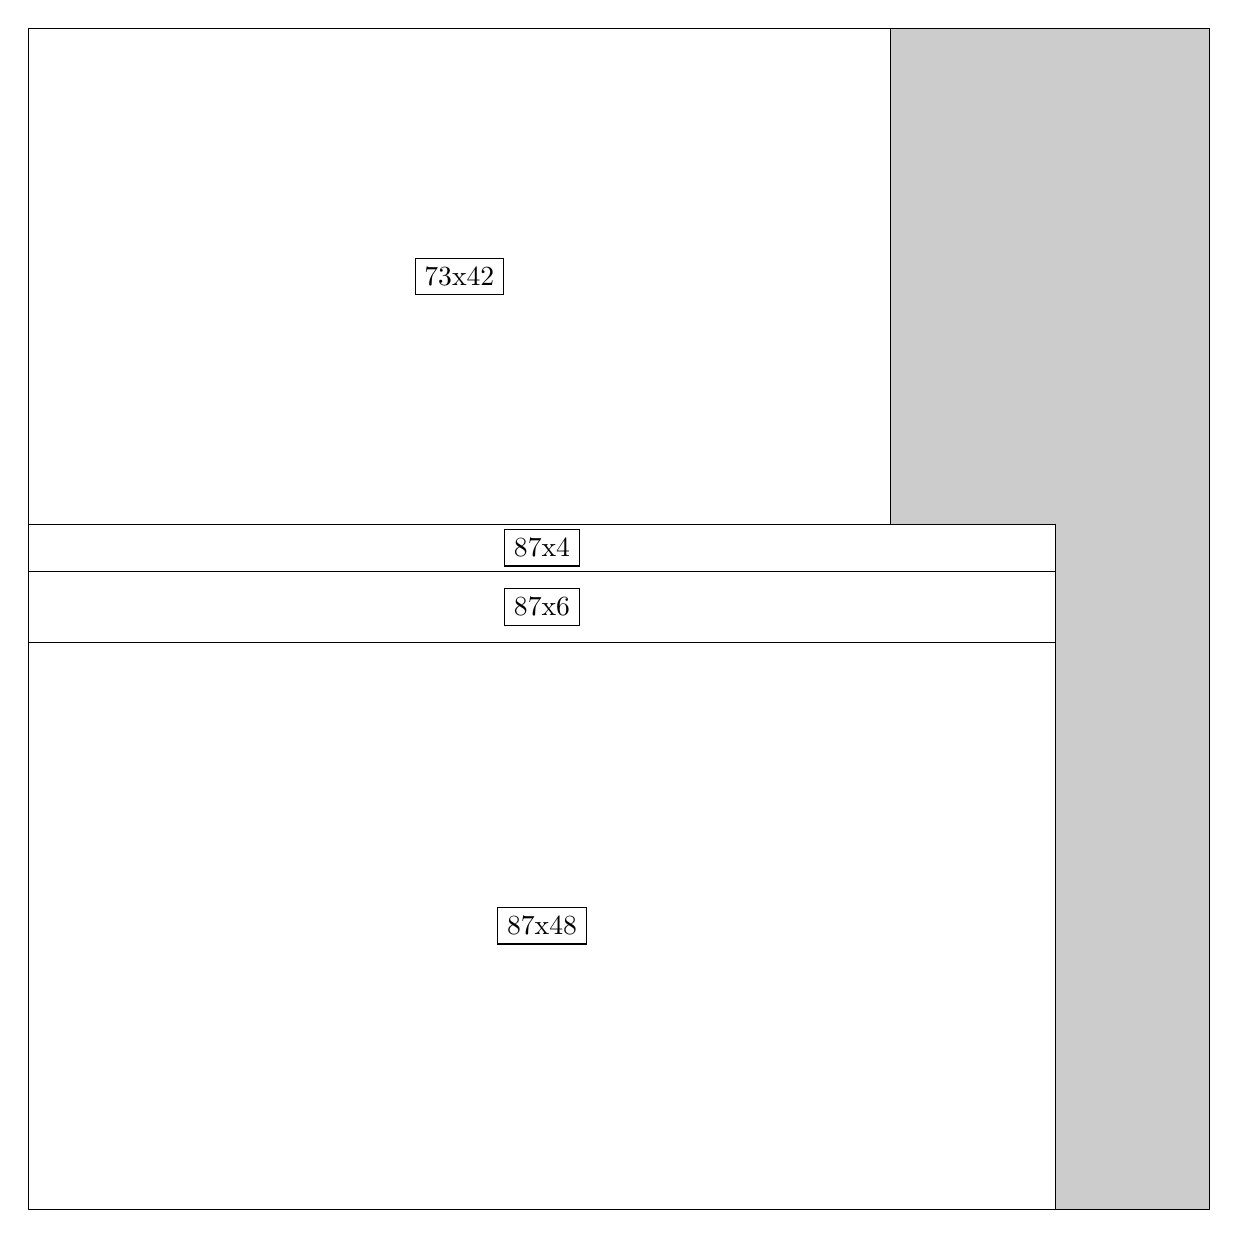
\begin{tikzpicture}[shorten >=1pt,scale=1.0,every node/.style={scale=1.0},->]
\tikzstyle{vertex}=[circle,fill=black!25,minimum size=14pt,inner sep=0pt]
\filldraw[fill=gray!40!white, draw=black] (0,0) rectangle (15.0,15.0);
\foreach \name/\x/\y/\w/\h in {87x48/0.0/0.0/13.049999999999999/7.199999999999999,73x42/0.0/8.7/10.95/6.3,87x6/0.0/7.199999999999999/13.049999999999999/0.8999999999999999,87x4/0.0/8.1/13.049999999999999/0.6}
\filldraw[fill=white!40!white, draw=black] (\x,\y) rectangle node[draw] (\name) {\name} ++(\w,\h);
\end{tikzpicture}


w =87 , h =48 , x =0 , y =0 , v =4176
\par
w =73 , h =42 , x =0 , y =58 , v =3066
\par
w =87 , h =6 , x =0 , y =48 , v =522
\par
w =87 , h =4 , x =0 , y =54 , v =348
\par
\newpage


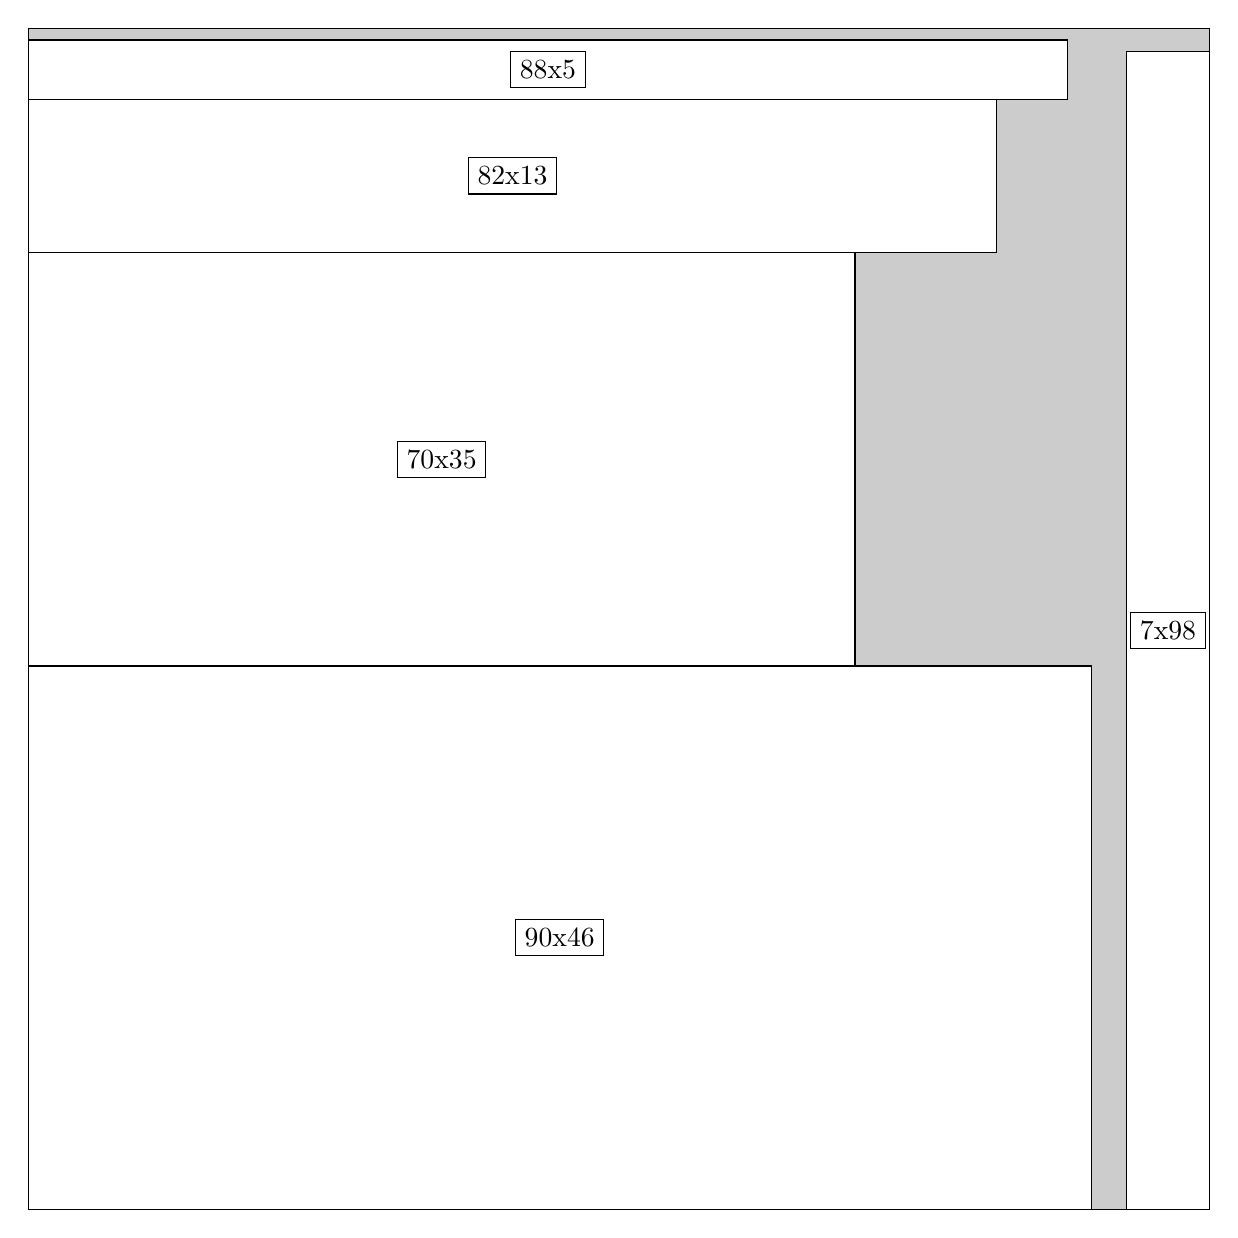
\begin{tikzpicture}[shorten >=1pt,scale=1.0,every node/.style={scale=1.0},->]
\tikzstyle{vertex}=[circle,fill=black!25,minimum size=14pt,inner sep=0pt]
\filldraw[fill=gray!40!white, draw=black] (0,0) rectangle (15.0,15.0);
\foreach \name/\x/\y/\w/\h in {90x46/0.0/0.0/13.5/6.8999999999999995,70x35/0.0/6.8999999999999995/10.5/5.25,82x13/0.0/12.15/12.299999999999999/1.95,7x98/13.95/0.0/1.05/14.7,88x5/0.0/14.1/13.2/0.75}
\filldraw[fill=white!40!white, draw=black] (\x,\y) rectangle node[draw] (\name) {\name} ++(\w,\h);
\end{tikzpicture}


w =90 , h =46 , x =0 , y =0 , v =4140
\par
w =70 , h =35 , x =0 , y =46 , v =2450
\par
w =82 , h =13 , x =0 , y =81 , v =1066
\par
w =7 , h =98 , x =93 , y =0 , v =686
\par
w =88 , h =5 , x =0 , y =94 , v =440
\par
\newpage


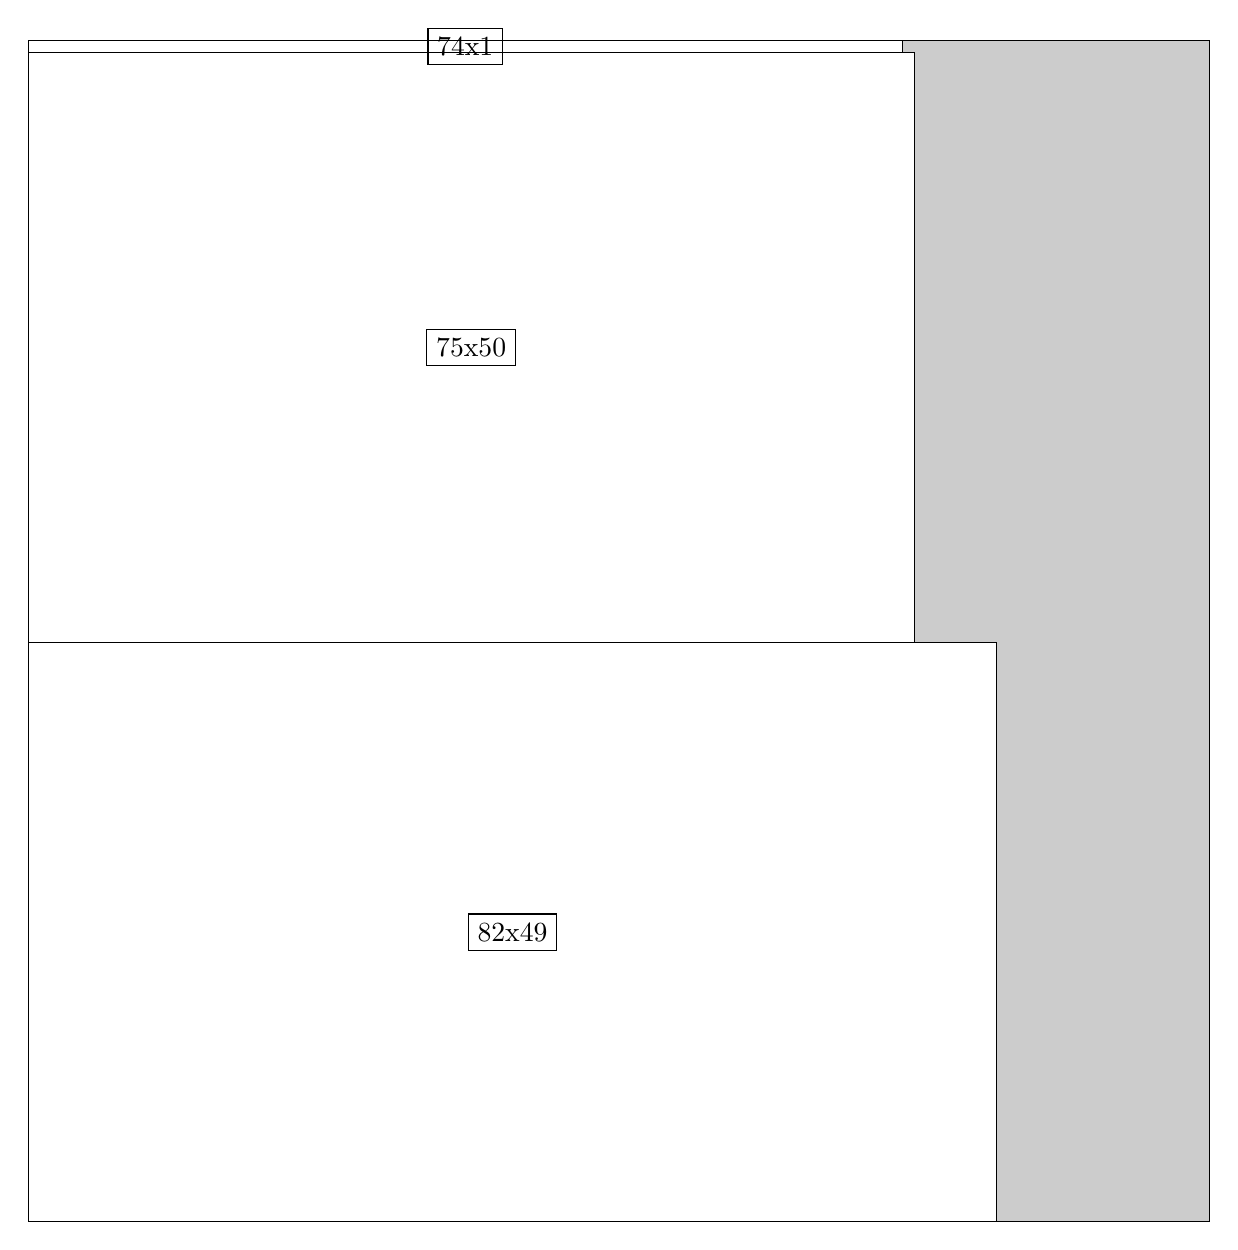
\begin{tikzpicture}[shorten >=1pt,scale=1.0,every node/.style={scale=1.0},->]
\tikzstyle{vertex}=[circle,fill=black!25,minimum size=14pt,inner sep=0pt]
\filldraw[fill=gray!40!white, draw=black] (0,0) rectangle (15.0,15.0);
\foreach \name/\x/\y/\w/\h in {82x49/0.0/0.0/12.299999999999999/7.35,75x50/0.0/7.35/11.25/7.5,74x1/0.0/14.85/11.1/0.15}
\filldraw[fill=white!40!white, draw=black] (\x,\y) rectangle node[draw] (\name) {\name} ++(\w,\h);
\end{tikzpicture}


w =82 , h =49 , x =0 , y =0 , v =4018
\par
w =75 , h =50 , x =0 , y =49 , v =3750
\par
w =74 , h =1 , x =0 , y =99 , v =74
\par
\newpage


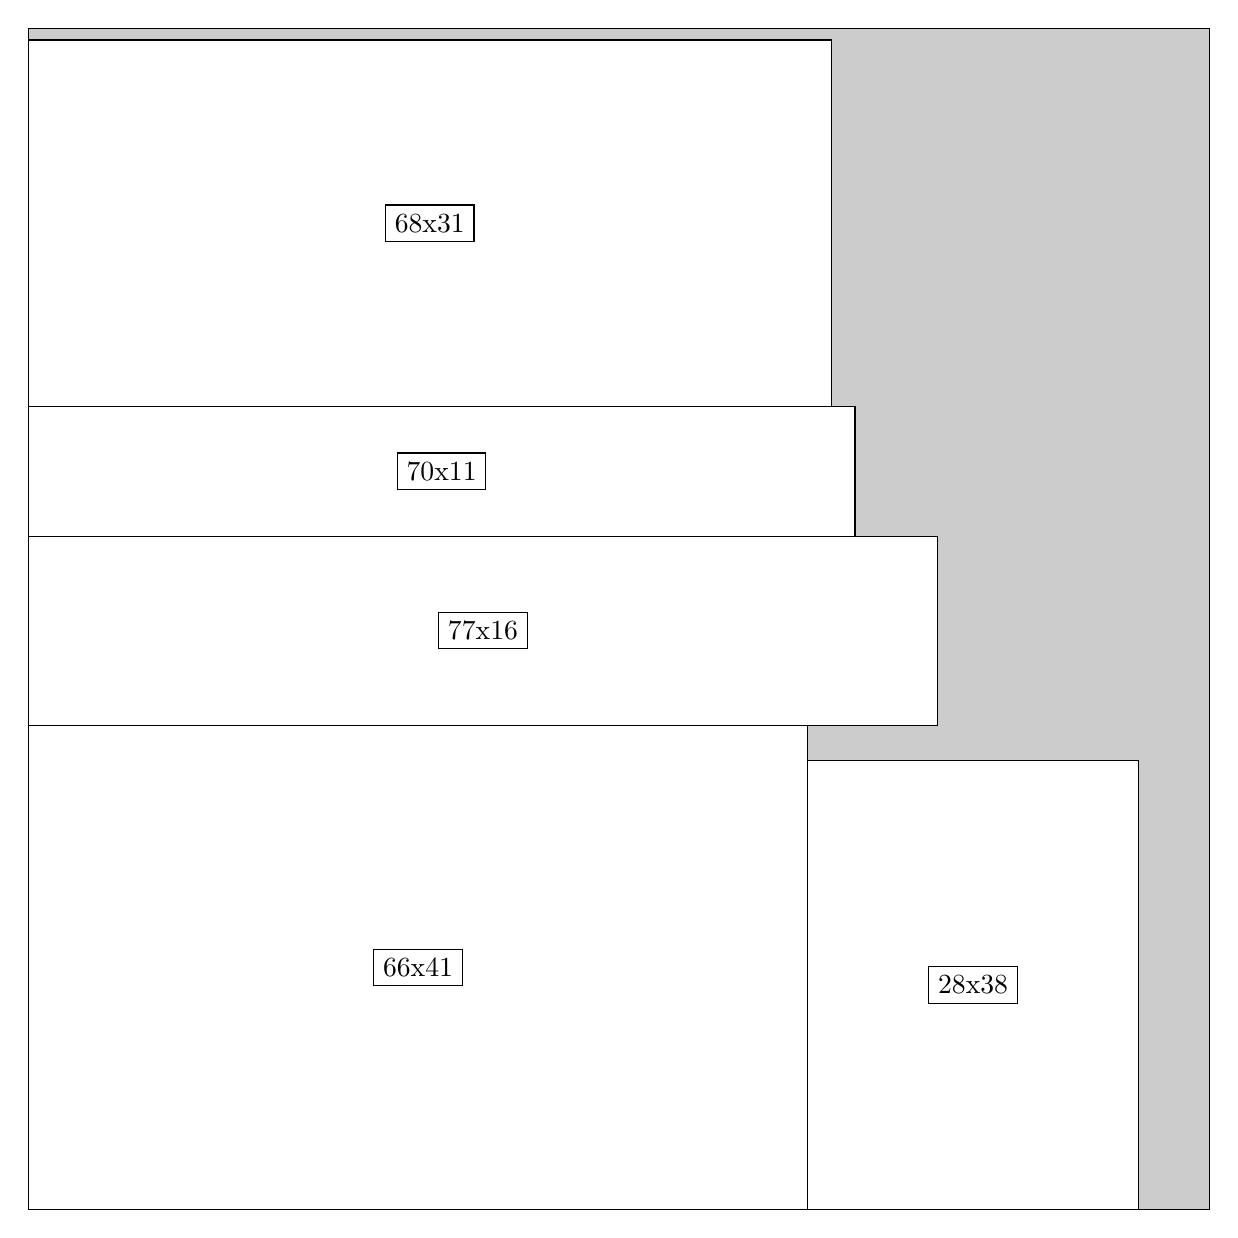
\begin{tikzpicture}[shorten >=1pt,scale=1.0,every node/.style={scale=1.0},->]
\tikzstyle{vertex}=[circle,fill=black!25,minimum size=14pt,inner sep=0pt]
\filldraw[fill=gray!40!white, draw=black] (0,0) rectangle (15.0,15.0);
\foreach \name/\x/\y/\w/\h in {70x11/0.0/8.549999999999999/10.5/1.65,66x41/0.0/0.0/9.9/6.1499999999999995,68x31/0.0/10.2/10.2/4.6499999999999995,77x16/0.0/6.1499999999999995/11.549999999999999/2.4,28x38/9.9/0.0/4.2/5.7}
\filldraw[fill=white!40!white, draw=black] (\x,\y) rectangle node[draw] (\name) {\name} ++(\w,\h);
\end{tikzpicture}


w =70 , h =11 , x =0 , y =57 , v =770
\par
w =66 , h =41 , x =0 , y =0 , v =2706
\par
w =68 , h =31 , x =0 , y =68 , v =2108
\par
w =77 , h =16 , x =0 , y =41 , v =1232
\par
w =28 , h =38 , x =66 , y =0 , v =1064
\par
\newpage


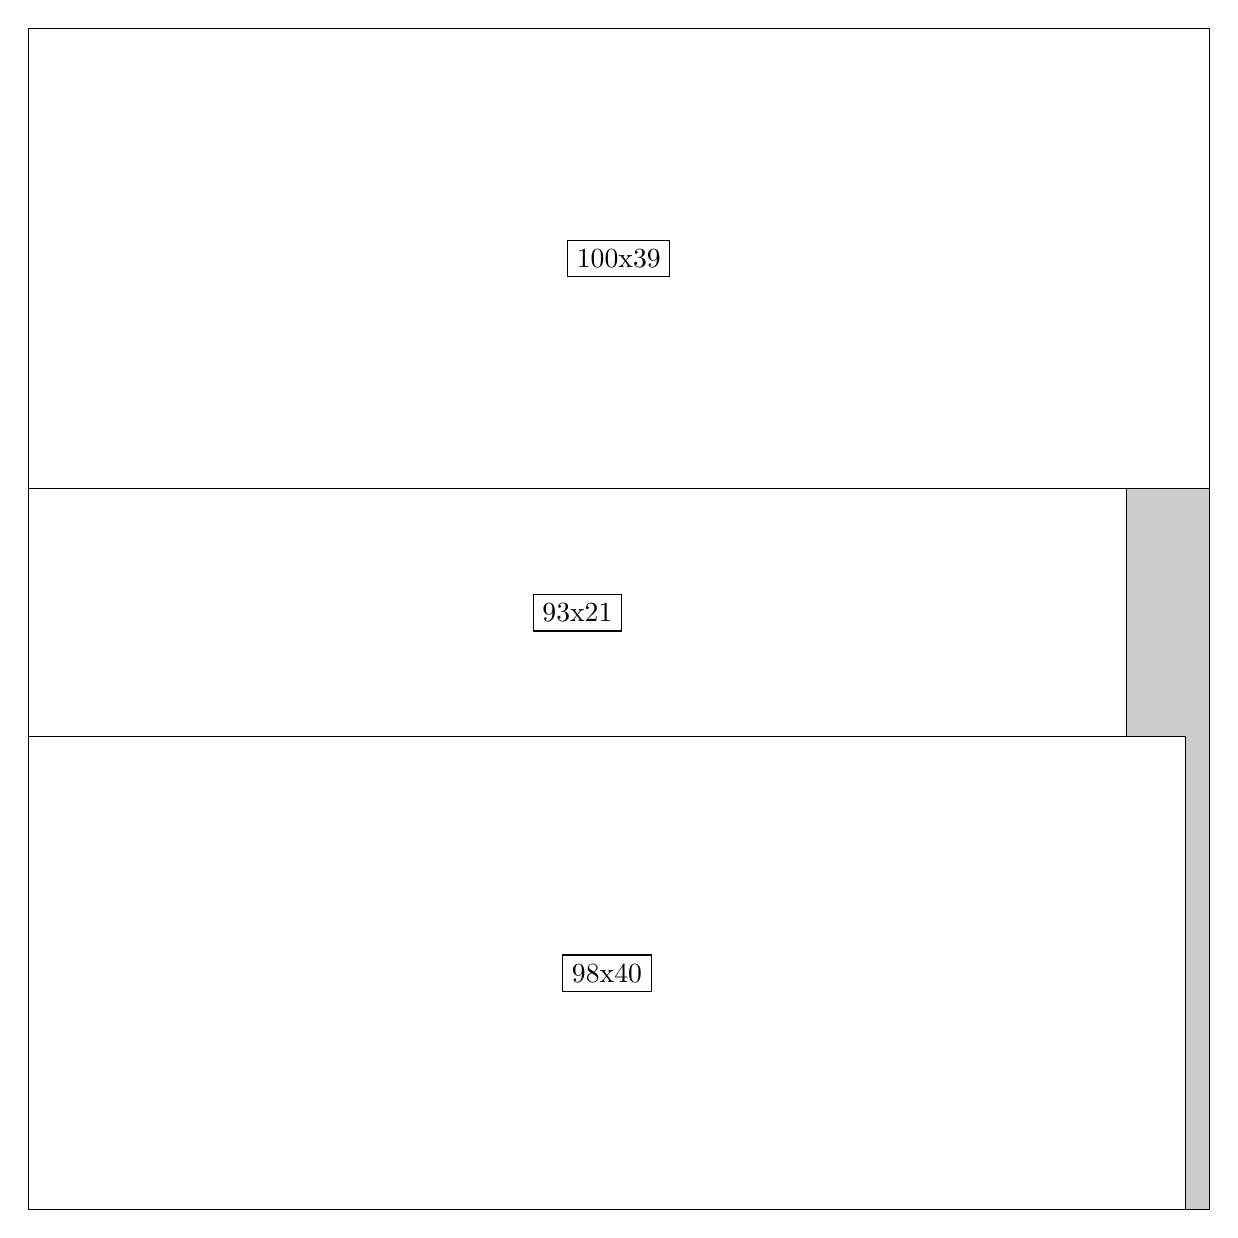
\begin{tikzpicture}[shorten >=1pt,scale=1.0,every node/.style={scale=1.0},->]
\tikzstyle{vertex}=[circle,fill=black!25,minimum size=14pt,inner sep=0pt]
\filldraw[fill=gray!40!white, draw=black] (0,0) rectangle (15.0,15.0);
\foreach \name/\x/\y/\w/\h in {98x40/0.0/0.0/14.7/6.0,100x39/0.0/9.15/15.0/5.85,93x21/0.0/6.0/13.95/3.15}
\filldraw[fill=white!40!white, draw=black] (\x,\y) rectangle node[draw] (\name) {\name} ++(\w,\h);
\end{tikzpicture}


w =98 , h =40 , x =0 , y =0 , v =3920
\par
w =100 , h =39 , x =0 , y =61 , v =3900
\par
w =93 , h =21 , x =0 , y =40 , v =1953
\par
\newpage


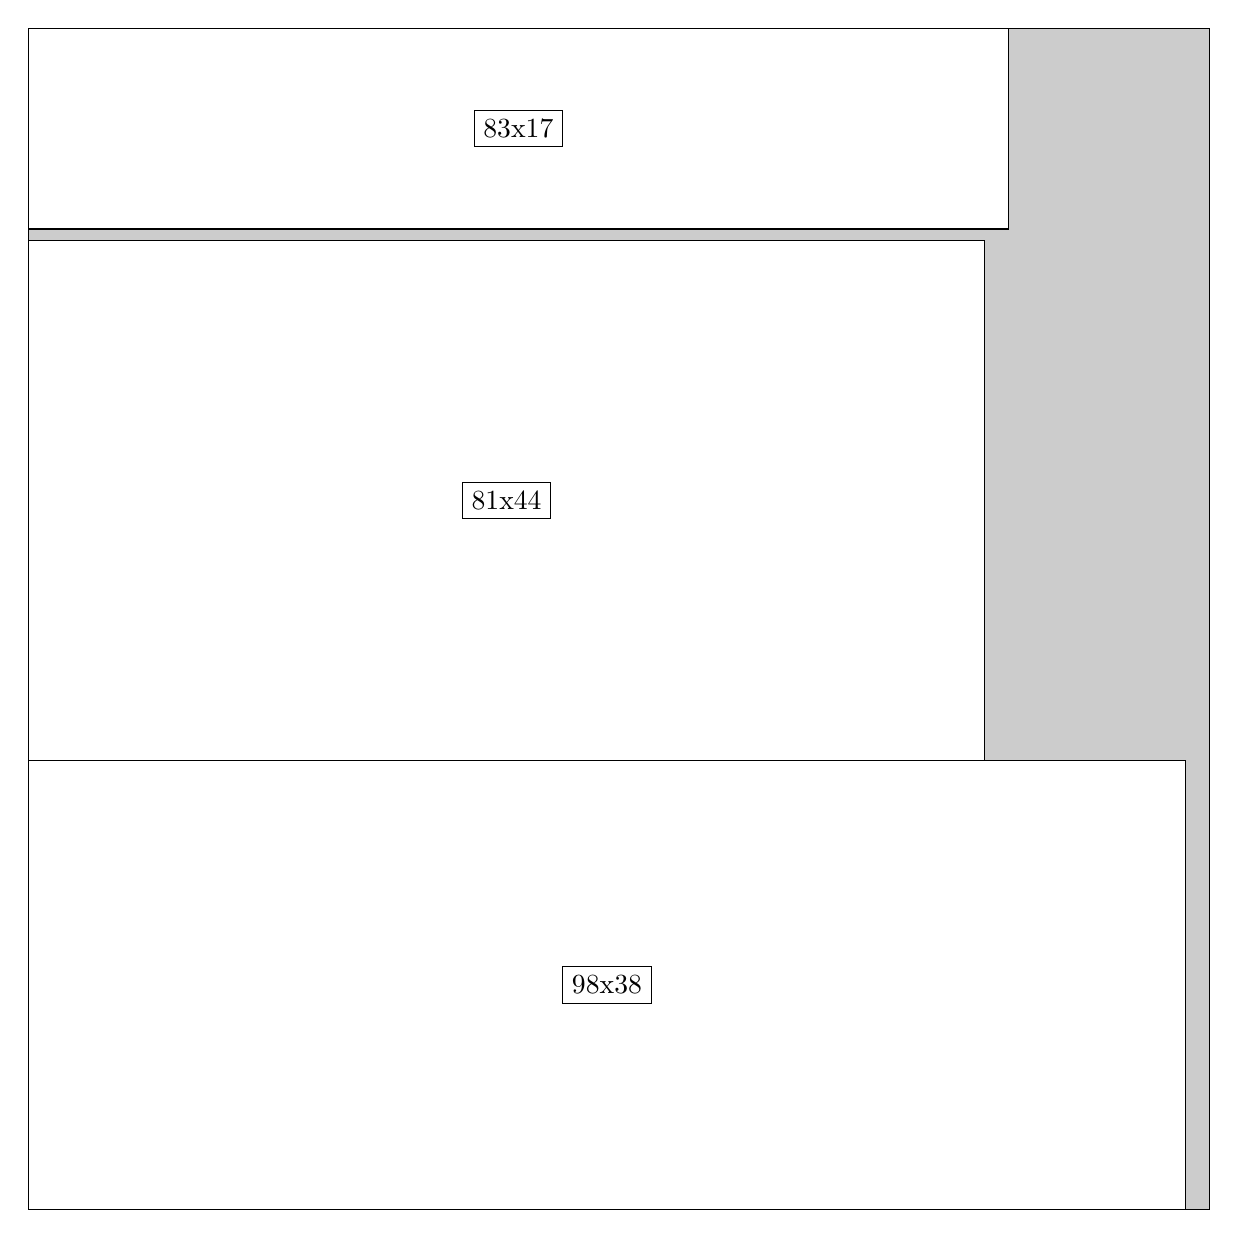
\begin{tikzpicture}[shorten >=1pt,scale=1.0,every node/.style={scale=1.0},->]
\tikzstyle{vertex}=[circle,fill=black!25,minimum size=14pt,inner sep=0pt]
\filldraw[fill=gray!40!white, draw=black] (0,0) rectangle (15.0,15.0);
\foreach \name/\x/\y/\w/\h in {98x38/0.0/0.0/14.7/5.7,81x44/0.0/5.7/12.15/6.6,83x17/0.0/12.45/12.45/2.55}
\filldraw[fill=white!40!white, draw=black] (\x,\y) rectangle node[draw] (\name) {\name} ++(\w,\h);
\end{tikzpicture}


w =98 , h =38 , x =0 , y =0 , v =3724
\par
w =81 , h =44 , x =0 , y =38 , v =3564
\par
w =83 , h =17 , x =0 , y =83 , v =1411
\par
\newpage


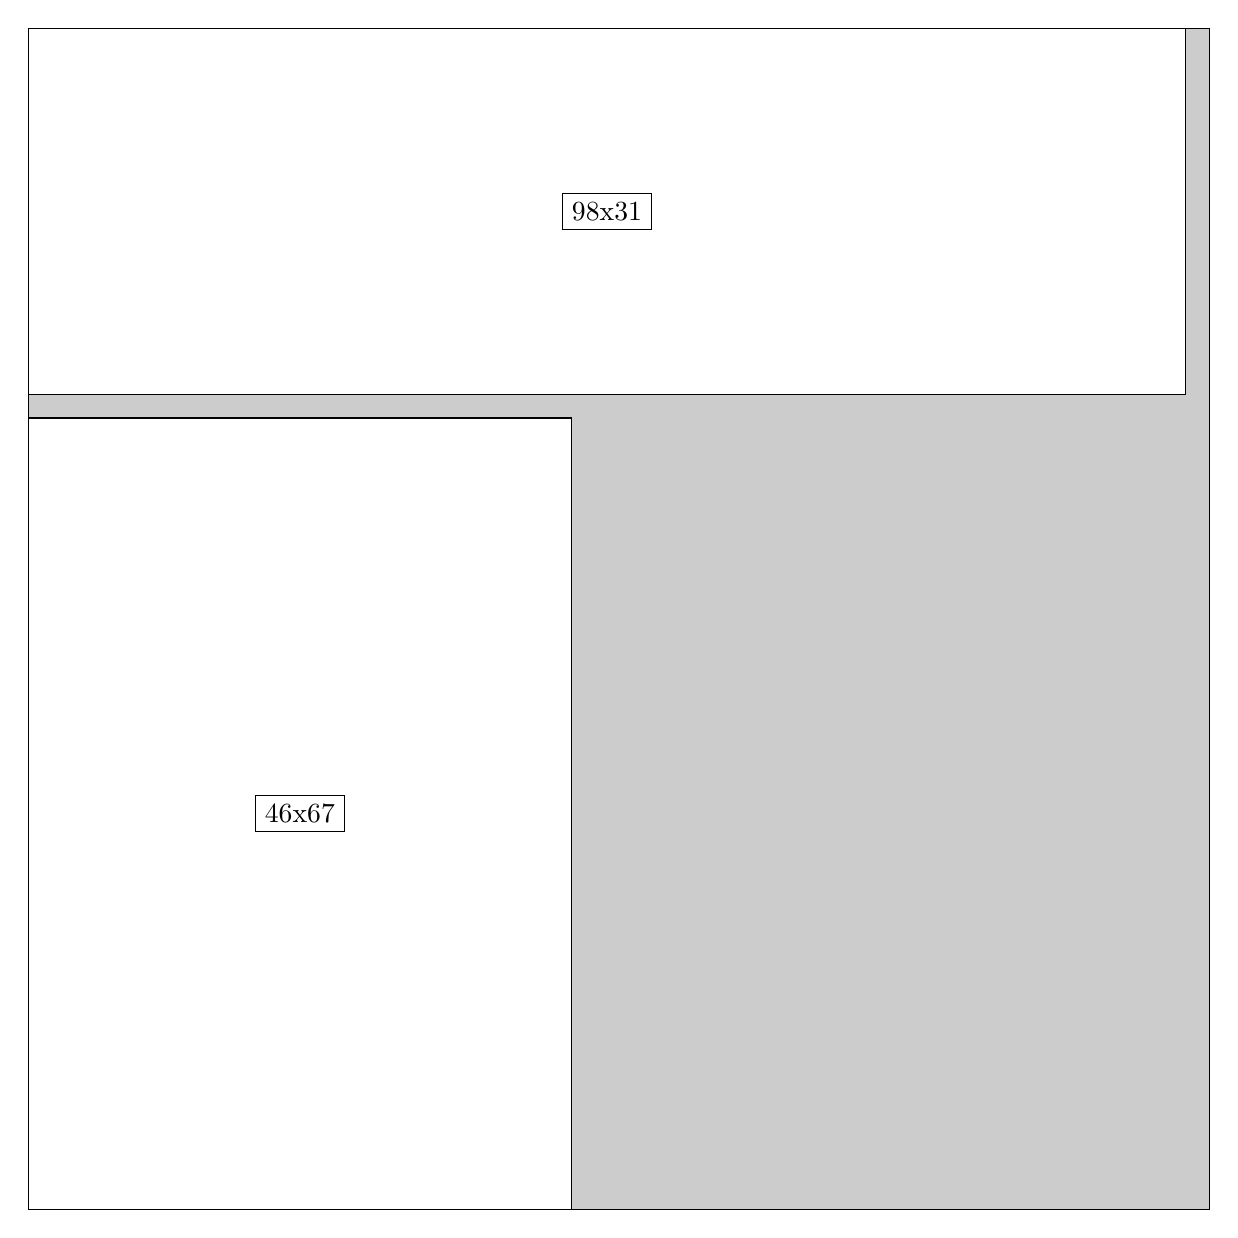
\begin{tikzpicture}[shorten >=1pt,scale=1.0,every node/.style={scale=1.0},->]
\tikzstyle{vertex}=[circle,fill=black!25,minimum size=14pt,inner sep=0pt]
\filldraw[fill=gray!40!white, draw=black] (0,0) rectangle (15.0,15.0);
\foreach \name/\x/\y/\w/\h in {46x67/0.0/0.0/6.8999999999999995/10.049999999999999,98x31/0.0/10.35/14.7/4.6499999999999995}
\filldraw[fill=white!40!white, draw=black] (\x,\y) rectangle node[draw] (\name) {\name} ++(\w,\h);
\end{tikzpicture}


w =46 , h =67 , x =0 , y =0 , v =3082
\par
w =98 , h =31 , x =0 , y =69 , v =3038
\par
\newpage


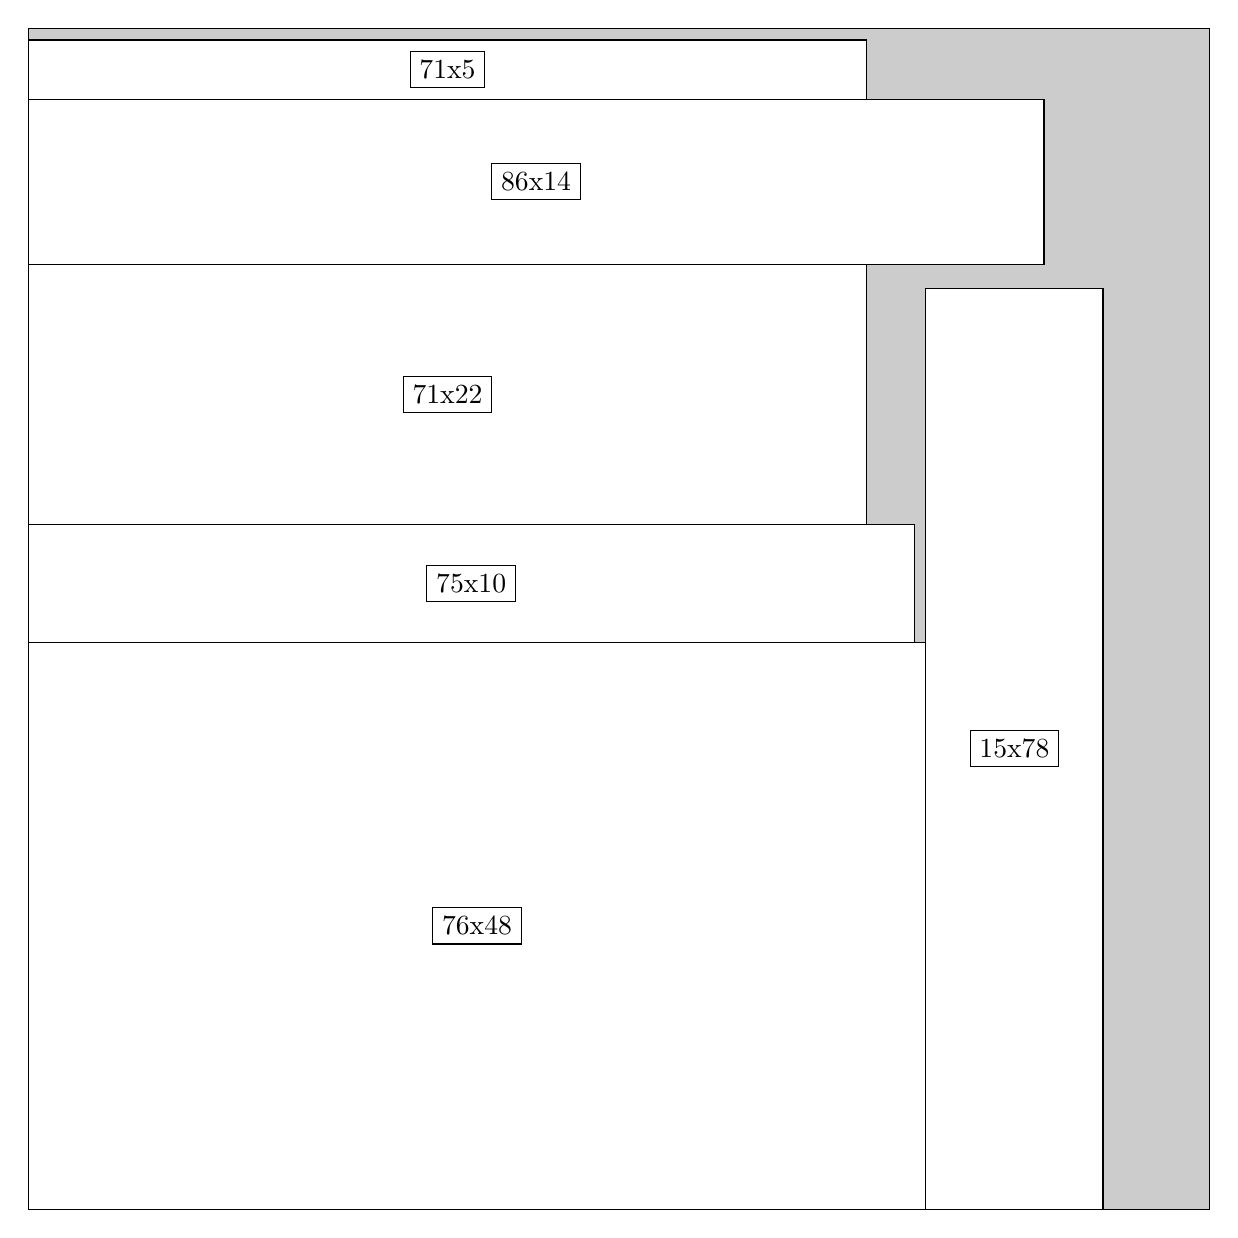
\begin{tikzpicture}[shorten >=1pt,scale=1.0,every node/.style={scale=1.0},->]
\tikzstyle{vertex}=[circle,fill=black!25,minimum size=14pt,inner sep=0pt]
\filldraw[fill=gray!40!white, draw=black] (0,0) rectangle (15.0,15.0);
\foreach \name/\x/\y/\w/\h in {76x48/0.0/0.0/11.4/7.199999999999999,75x10/0.0/7.199999999999999/11.25/1.5,71x22/0.0/8.7/10.65/3.3,86x14/0.0/12.0/12.9/2.1,15x78/11.4/0.0/2.25/11.7,71x5/0.0/14.1/10.65/0.75}
\filldraw[fill=white!40!white, draw=black] (\x,\y) rectangle node[draw] (\name) {\name} ++(\w,\h);
\end{tikzpicture}


w =76 , h =48 , x =0 , y =0 , v =3648
\par
w =75 , h =10 , x =0 , y =48 , v =750
\par
w =71 , h =22 , x =0 , y =58 , v =1562
\par
w =86 , h =14 , x =0 , y =80 , v =1204
\par
w =15 , h =78 , x =76 , y =0 , v =1170
\par
w =71 , h =5 , x =0 , y =94 , v =355
\par
\newpage


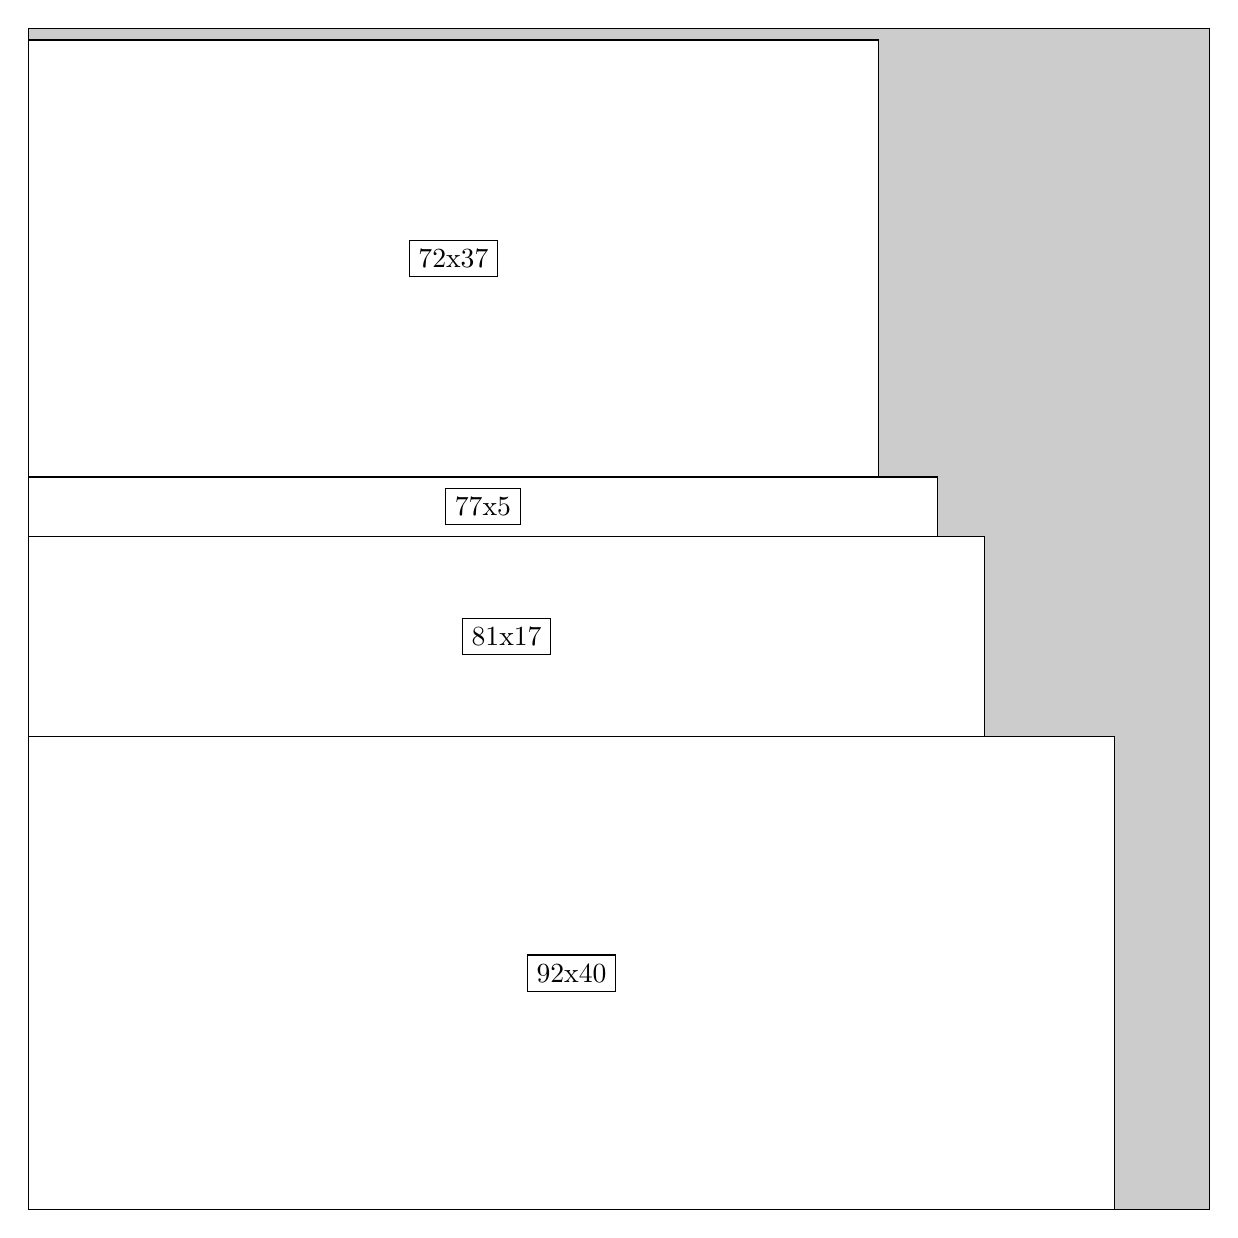
\begin{tikzpicture}[shorten >=1pt,scale=1.0,every node/.style={scale=1.0},->]
\tikzstyle{vertex}=[circle,fill=black!25,minimum size=14pt,inner sep=0pt]
\filldraw[fill=gray!40!white, draw=black] (0,0) rectangle (15.0,15.0);
\foreach \name/\x/\y/\w/\h in {92x40/0.0/0.0/13.799999999999999/6.0,72x37/0.0/9.299999999999999/10.799999999999999/5.55,81x17/0.0/6.0/12.15/2.55,77x5/0.0/8.549999999999999/11.549999999999999/0.75}
\filldraw[fill=white!40!white, draw=black] (\x,\y) rectangle node[draw] (\name) {\name} ++(\w,\h);
\end{tikzpicture}


w =92 , h =40 , x =0 , y =0 , v =3680
\par
w =72 , h =37 , x =0 , y =62 , v =2664
\par
w =81 , h =17 , x =0 , y =40 , v =1377
\par
w =77 , h =5 , x =0 , y =57 , v =385
\par
\newpage


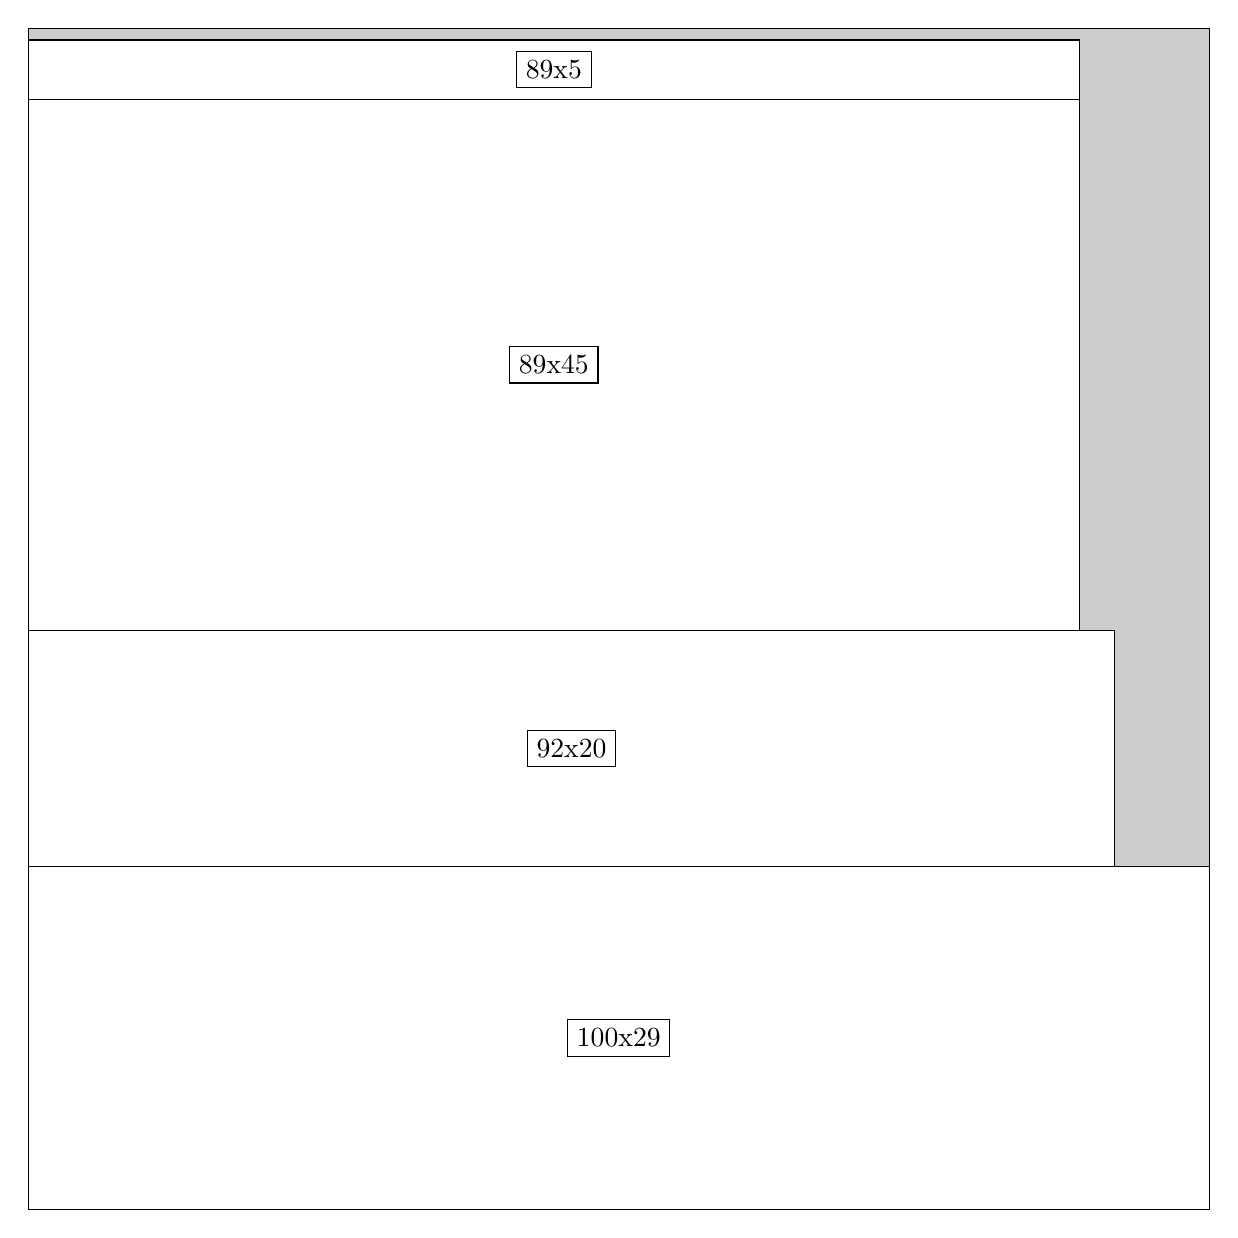
\begin{tikzpicture}[shorten >=1pt,scale=1.0,every node/.style={scale=1.0},->]
\tikzstyle{vertex}=[circle,fill=black!25,minimum size=14pt,inner sep=0pt]
\filldraw[fill=gray!40!white, draw=black] (0,0) rectangle (15.0,15.0);
\foreach \name/\x/\y/\w/\h in {100x29/0.0/0.0/15.0/4.35,92x20/0.0/4.35/13.799999999999999/3.0,89x45/0.0/7.35/13.35/6.75,89x5/0.0/14.1/13.35/0.75}
\filldraw[fill=white!40!white, draw=black] (\x,\y) rectangle node[draw] (\name) {\name} ++(\w,\h);
\end{tikzpicture}


w =100 , h =29 , x =0 , y =0 , v =2900
\par
w =92 , h =20 , x =0 , y =29 , v =1840
\par
w =89 , h =45 , x =0 , y =49 , v =4005
\par
w =89 , h =5 , x =0 , y =94 , v =445
\par
\newpage


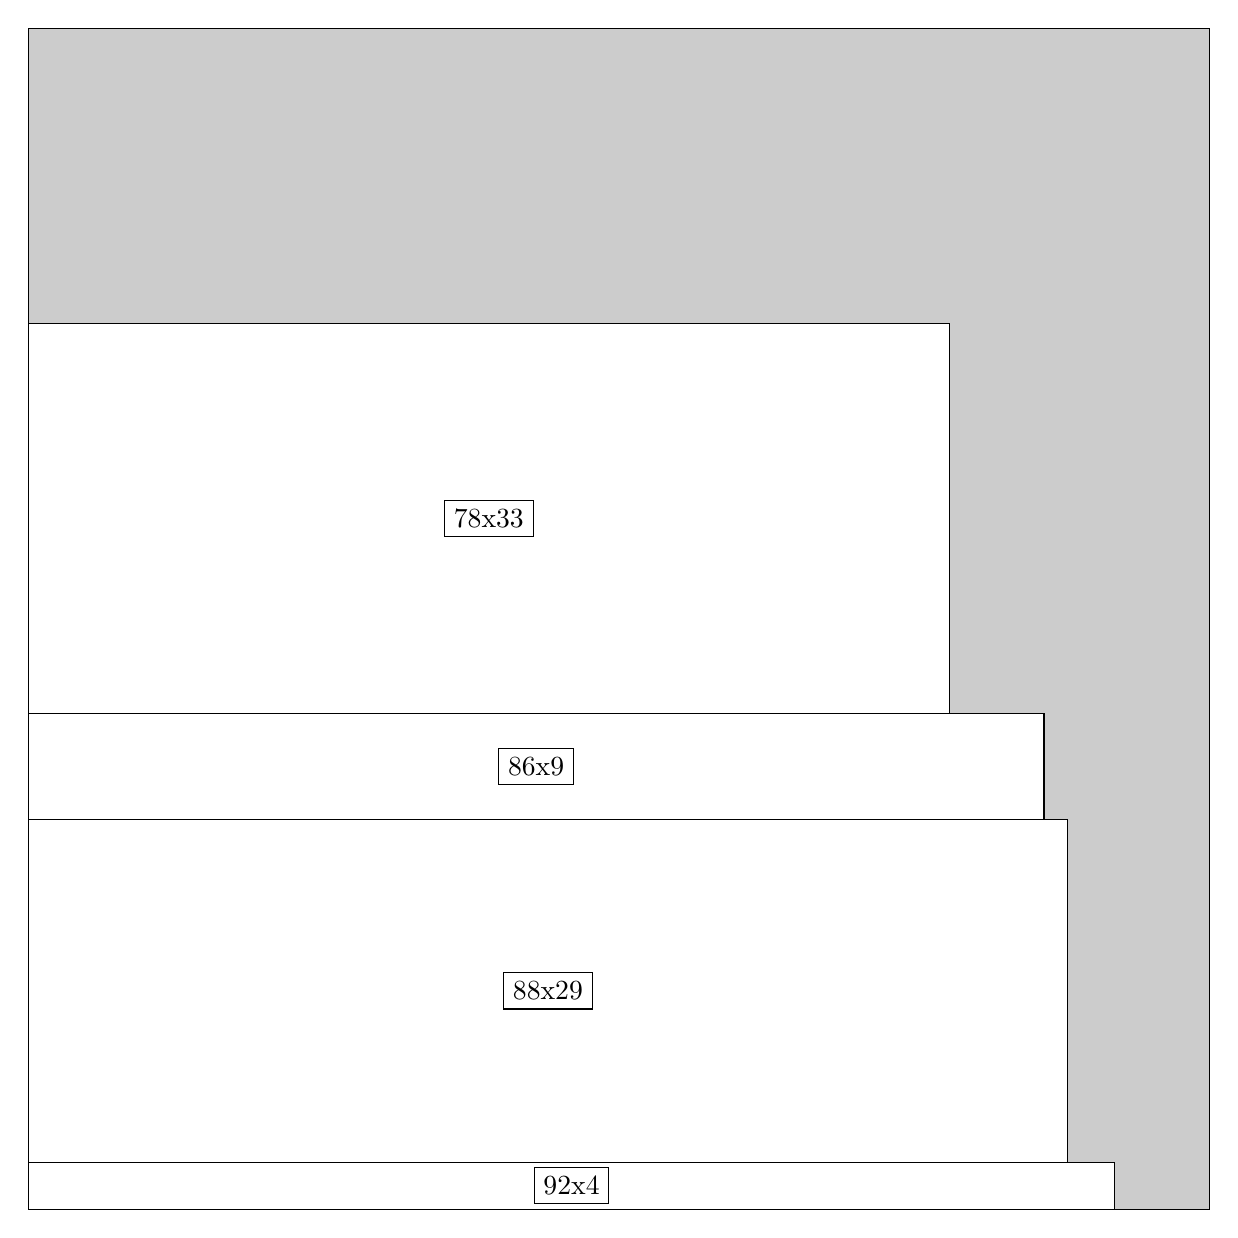
\begin{tikzpicture}[shorten >=1pt,scale=1.0,every node/.style={scale=1.0},->]
\tikzstyle{vertex}=[circle,fill=black!25,minimum size=14pt,inner sep=0pt]
\filldraw[fill=gray!40!white, draw=black] (0,0) rectangle (15.0,15.0);
\foreach \name/\x/\y/\w/\h in {78x33/0.0/6.3/11.7/4.95,88x29/0.0/0.6/13.2/4.35,86x9/0.0/4.95/12.9/1.3499999999999999,92x4/0.0/0.0/13.799999999999999/0.6}
\filldraw[fill=white!40!white, draw=black] (\x,\y) rectangle node[draw] (\name) {\name} ++(\w,\h);
\end{tikzpicture}


w =78 , h =33 , x =0 , y =42 , v =2574
\par
w =88 , h =29 , x =0 , y =4 , v =2552
\par
w =86 , h =9 , x =0 , y =33 , v =774
\par
w =92 , h =4 , x =0 , y =0 , v =368
\par
\newpage


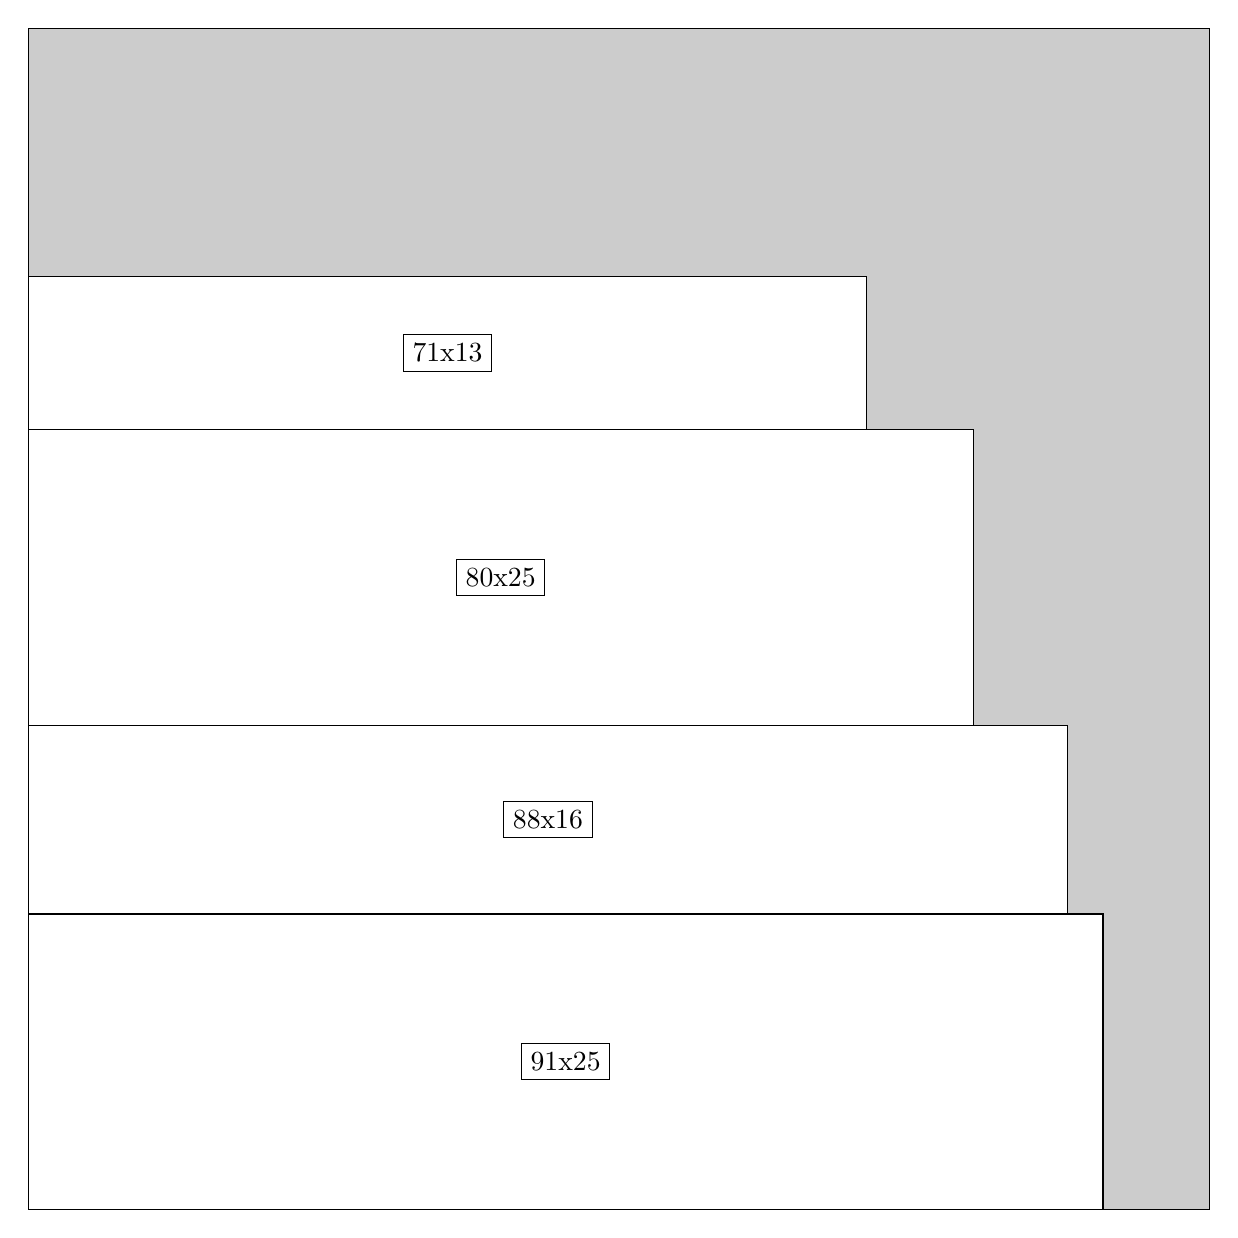
\begin{tikzpicture}[shorten >=1pt,scale=1.0,every node/.style={scale=1.0},->]
\tikzstyle{vertex}=[circle,fill=black!25,minimum size=14pt,inner sep=0pt]
\filldraw[fill=gray!40!white, draw=black] (0,0) rectangle (15.0,15.0);
\foreach \name/\x/\y/\w/\h in {91x25/0.0/0.0/13.65/3.75,80x25/0.0/6.1499999999999995/12.0/3.75,88x16/0.0/3.75/13.2/2.4,71x13/0.0/9.9/10.65/1.95}
\filldraw[fill=white!40!white, draw=black] (\x,\y) rectangle node[draw] (\name) {\name} ++(\w,\h);
\end{tikzpicture}


w =91 , h =25 , x =0 , y =0 , v =2275
\par
w =80 , h =25 , x =0 , y =41 , v =2000
\par
w =88 , h =16 , x =0 , y =25 , v =1408
\par
w =71 , h =13 , x =0 , y =66 , v =923
\par
\newpage


\end{document}